%Gilmore Space LaTeX template
%Rory Kelly ~ 21 Nov 2024
%Needed for ?. Must come before document class
\RequirePackage{pdfmanagement-testphase}
\DeclareDocumentMetadata{}
\documentclass[12pt]{article}
%
\input{preamble}
%
\setmainfont{Arial}[
]
%
\definecolor{AtmoBlue}{HTML}{00aeef}
\definecolor{DeepSpace}{HTML}{0c004b}
\definecolor{Rocket}{HTML}{c9cacc}
\definecolor{Titles}{HTML}{2f5496}
\definecolor{Table_Light}{HTML}{deeaf6}
\definecolor{Table_Dark}{HTML}{bdd6ee}
\definecolor{Table_Title}{HTML}{5b9bd5}
%
\titleformat{\section}
{\color{Titles}\normalfont\Large}
{\color{Titles}\thesection}{1em}{}
\titleformat{\subsection}
{\color{Titles}\normalfont\large}
{\color{Titles}\thesubsection}{1em}{}
\titleformat{\subsubsection}
{\color{Titles}\normalfont}
{\color{Titles}\thesubsubsection}{1em}{}
%
%%%%%%%%%%%%%%%%%%%%%%%%%%%%%%%%%%%%%%%%%%%%%%%%%%%%%%%%%%%%%%%%%%%%%%%
%%%%%%%%%%%%%%%%%%%%%%%%%%%%%%%%%%%%%%%%%%%%%%%%%%%%%%%%%%%%%%%%%%%%%%%
%%%%%%%%%%%%%%%%%%%%%%%%%%%%%%%%%%%%%%%%%%%%%%%%%%%%%%%%%%%%%%%%%%%%%%%
%
% IMPORTANT, PUT THE DOCUMENT INFORMATION HERE!!!
\newcommand{\DocumentID}{000-00000}
\newcommand{\VersionID}{ABCD}
\newcommand{\PublishID}{\today}
%
\pagestyle{fancy}
\lhead{\scriptsize CHARON Aerodynamics}
\rhead{\scriptsize \DocumentID \\ \VersionID}
\chead{\includegraphics[width=4cm]{logo.png}}
\lfoot{}
\rfoot{\scriptsize Page \thepage\ of \pageref{LastPage}}
\cfoot{\scriptsize Private and Confidential © 2024 Gilmour Space}
\renewcommand{\headrulewidth}{0.2pt}
\renewcommand{\footrulewidth}{0.2pt}
% LC: prolongate header and foot line
\renewcommand{\headrule}{\hrule width \textwidth} 
\renewcommand{\footrule}{\hrule width \textwidth} 
%
\geometry{
    a4paper,
    total={170mm,257mm},
    margin=1in,
}
%
% \pagenumbering{Roman}
%
%Turn of the LaTeX indents
\setlength{\parindent}{0pt}
\setlength{\parskip}{5pt}
 %
%Totally forgot what this was for
\makeatletter
\setlength{\@fptop}{0pt}
\makeatother
%
%Add the title page background
\AddToShipoutPictureBG*{
    \put(0,0){
        \parbox[b][\paperheight]{\paperwidth}{%
            \vfill
            \centering
            \transparent{0.25}\includegraphics[width=15cm]{./background.png}%
            \vfill
        }
    }
}

\title{Charon jet-ON}
\author{Lorenzo Campoli}
\date{\today}
%
\begin{document}
%
\setmainfont{Arial}
%
\maketitle
%
\renewcommand{\arraystretch}{1.5} % Adjust row height
\setlength{\tabcolsep}{8pt}       % Adjust column spacing

\begin{center}
\resizebox{\textwidth}{!}{ % Automatically adjust table width to fit the page
\begin{tabular}{m{3.5cm}|m{4cm}m{7.5cm}m{4.5cm}}
%
                      & \textbf{NAME}           & \textbf{TITLE/ROLE} & \textbf{SIGNATURE} \\ \hline
\textbf{AUTHORED BY}  & Lorenzo Campoli         & Senior System Modelling Engineer    & \includegraphics[width=4cm]{signature/signature0.png} \\  
\textbf{REVIEWED BY}  & Matthew Pengelly        & Lead System Modelling Engineer    & \\ 
                      & Jonte Healy             & System Modelling Engineer II   & \\ 
\textbf{APPROVED BY}  & Smritee Darcy           & Optimus System Mechanical Engineer     & \\ \hline
\end{tabular}}
\end{center}

\begin{abstract}
\noindent In this work package, the the aerothermodynamics characterization of the Charon vehicle is numerically carried out. Several configurations are considered, specifically, \textbf{jetOFF/VernierOFF, jetOFF/VernierON, jetON/VernierOFF, jetON/VernierON}. The main outcome of this report is the aerodynamic coefficients as well as the pressure (average, minimum, maximum) and area-averaged heat flux on every patch identified as "of interest" for the selected flight trajectory points.
\end{abstract}
%
%\newpage
%\makenomenclature
%\newpage
%\printnomenclature
%\input{nomenclature}
%
\tableofcontents
%
%%%%%%%%%%%%%%%%%%%%%%%%%%%%%%%%%%%%%%%%%%%%%%
\section{Introduction}\label{sec:introduction}
%%%%%%%%%%%%%%%%%%%%%%%%%%%%%%%%%%%%%%%%%%%%%%
%
\begin{figure}[H]
    \centering
    \includegraphics[width=\linewidth]{figs/nozzle_exit_plane.png}
    \caption{Charon nozzle exit plane conditions calculated from RPA.}
    \label{fig:vernier-force}
\end{figure}
%
%%%%%%%%%%%%%%%%%%%%%%%%%%%%%%%%%%
\section{Method}\label{sec:method}
%%%%%%%%%%%%%%%%%%%%%%%%%%%%%%%%%%
ANSYS Fluent computes aerodynamic forces, moments, and their dimensionless coefficients using surface integrals of pressure and viscous stress over specified wall zones. These are essential for evaluating the performance of aerospace and automotive designs.

\subsection{Force Calculation}
The total force acting on a wall zone is obtained by integrating pressure and viscous stresses:

$$
\vec{F} = \int_{A} \left( -p \vec{n} + \vec{\tau} \right) dA
$$
where:
   
- $ p $: static pressure
    
- $ \vec{n} $: unit normal vector to the surface
    
- $ \vec{\tau} $: viscous stress vector
    
- $ A $: surface area of the selected wall(s)


\subsection{Moment Calculation}
The aerodynamic moment about a reference point $\vec{r}_0$ is given by:

$$
\vec{M} = \int_{A} \left( \vec{r} - \vec{r}_0 \right) \times \left( -p \vec{n} + \vec{\tau} \right) dA
$$
where:
    
- $ \vec{r} $: position vector of the surface element
    
- $ \vec{r}_0 $: moment reference point

\subsection{Dimensionless Aerodynamic Coefficients}
Fluent uses dynamic pressure $ q_\infty = \frac{1}{2} \rho_\infty V_\infty^2 $ to compute non-dimensional coefficients:

\subsubsection*{Drag Coefficient}
$$
C_D = \frac{F_D}{q_\infty S}
$$

\subsubsection*{Lift Coefficient}
$$
C_L = \frac{F_L}{q_\infty S}
$$

\subsubsection*{Side Force Coefficient}
$$
C_Y = \frac{F_Y}{q_\infty S}
$$

\subsubsection*{Pitching Moment Coefficient}
%%%%%%%%%%%%%%%%%%%%%%%%%%%%%%%%%%%%%%%%%%%%
$$
C_M = \frac{M}{q_\infty S c}
$$

where:
    
- $ F_D, F_L, F_Y $: drag, lift, and side-force components respectively
    
- $ M $: pitching moment
    
- $ q_\infty = \frac{1}{2} \rho_\infty V_\infty^2 $: freestream dynamic pressure
    
- $ \rho_\infty $: freestream density
    
- $ V_\infty $: freestream velocity
    
- $ S $: reference area
    
- $ c $: reference length (e.g., chord length)

\subsection{Summary Table}
%%%%%%%%%%%%%%%%%%%%%%%%%%
\begin{center}
\begin{tabular}{ll}
\hline
\textbf{Quantity} & \textbf{Formula} \\
\hline
Total Force & $ \vec{F} = \int_A (-p \vec{n} + \vec{\tau}) dA $ \\
Moment & $ \vec{M} = \int_A (\vec{r} - \vec{r}_0) \times (-p \vec{n} + \vec{\tau}) dA $ \\
Drag Coefficient & $ C_D = \frac{F_D}{\frac{1}{2} \rho_\infty V_\infty^2 S} $ \\
Lift Coefficient & $ C_L = \frac{F_L}{\frac{1}{2} \rho_\infty V_\infty^2 S} $ \\
Pitching Moment Coefficient & $ C_M = \frac{M}{\frac{1}{2} \rho_\infty V_\infty^2 S c} $ \\
\hline
\end{tabular}
\end{center}

\subsection{Reference Quantities}
%%%%%%%%%%%%%%%%%%%%%%%%%%%%%%%%%
These coefficients depend on reference values that can be set in Fluent under:

\begin{center}
    \texttt{Reports → Reference Values...}
\end{center}

Ensure appropriate values are defined for:
    
- Reference Area ($S$)
    
- Reference Length ($c$)
    
- Freestream Density ($\rho_\infty$)
    
- Freestream Velocity ($V_\infty$)

Table~\ref{tab:combined-reference-values} presents the reference values used for the numerical simulations at different times. %The values of the dynamic pressure, in the last column were calculated according to Equation~\ref{eq:qinf}.
%
%\begin{equation}
%    q = \frac{1}{2} \rho v^2    
%    \label{eq:qinf}
%\end{equation}

\begin{table}[H]
\centering
\caption{Reference Values for Various Test Cases.}
\label{tab:combined-reference-values}
\begin{tabular}{l|rrrrrrr}
\toprule
\textbf{Test Case} & $P_{\infty} [Pa]$ & $\rho_{\infty} (kg/m^3)$ & $V_{\infty} (m/s)$ & $S_{ref} (m^2)$ & $c_{ref} (m)$ & $q_{\infty} (kg/m \cdot s^2)$ \\
\midrule
TC035 & 67313 & 0.879731    & 212.8       & 0.44175 & 1.5 & 19961.2 \\
TC039 & 59538 & 0.7964      & 237.4       & 0.44175 & 1.5 & 22442.1 \\
TC060 & 28204 & 0.435       & 301         & 0.44175 & 1.5 & 19729.4 \\
TC065 & 22528 & 0.3622478   & 318         & 0.44175 & 1.5 & 18316 \\
TC072 & 16589 & 0.26675     & 354.2       & 0.44175 & 1.5 & 16784.7 \\
TC136 & 232 & 0.003178    & 1683        & 0.44175 & 1.5 & 4500.8 \\
\bottomrule
\end{tabular}
\end{table}

\subsection{Definition of Heat Transfer Coefficient (HTC)}
%%%%%%%%%%%%%%%%%%%%%%%%%%%%%%%%%%%%%%%%%%%%%%%%%%%%%%%%%%

The \textit{heat transfer coefficient} (HTC) is a characteristic of the flow that quantifies the ability of a fluid to convect energy from solid walls:

$$
\text{HTC} = \frac{q_{\text{wall}}}{T_{\text{wall}} - T_{\text{ref}}}
$$

For forced convection flows, HTC is traditionally expressed as a function of velocity, fluid properties, and geometry:

$$
\text{Nu} = \frac{\text{HTC} \cdot L}{k} = \text{Nu(Re, Pr)}
$$

This formulation assumes $ T_{\text{ref}} $ is a bulk (mass-averaged or "mixing cup") temperature. Under constant property assumptions, this definition renders HTC independent of the thermal field.

\subsection{Methods to Calculate HTC in ANSYS Fluent}
%%%%%%%%%%%%%%%%%%%%%%%%%%%%%%%%%%%%%%%%%%%%%%%%%%%%%
%https://innovationspace.ansys.com/courses/courses/topics-in-convective-heat-transfer-simulations/lessons/defining-heat-transfer-coefficient/
The "Surface Heat Transfer Coefficient" is calculated with "wall temperature", "total surface heat flux" and a "reference temperature". This reference temperature is a global value used on all faces. The accuracy of the surface htc (heat transfer coefficient) depends on the accuracy of the simulation and this reference or bulk temperature. For complex geometries it can be next to impossible to set a good reference temperature for large surfaces. Nevertheless, this is the parameter that is used by most Nusselt number correlations. The "Wall Func. Heat Tran. Coef." depends on the local solution of the flow field in a cell next to a wall. It is completely independent of the surface heat flux. Therefore it exists also for adiabatic walls. Since wall function htc depends on the turbulence model and the local temperature in the cell and at the wall the value has a strong dependency on the mesh resolution. It is quite rare that this parameter is used to judge the results of a simulation. For a mesh with large $y^+$ values and a reasonable reference temperature both parameters have similar results.

There are at least three methods to compute HTC in ANSYS Fluent.

\subsubsection{Method 1: Using Reference Temperature}
%%%%%%%%%%%%%%%%%%%%%%%%%%%%%%%%%%%%%%%%%%%%%%%%%%%%%

\begin{equation}
    \text{HTC} = \frac{q_{\text{wall}}}{T_{\text{wall}} - T_{\text{ref}}}
    \label{eq:htc}
\end{equation}

Here, $ T_{\text{ref}} $ is defined by the user under \texttt{Report $\rightarrow$ Reference Values}. This HTC value is directly available in Fluent under \texttt{Wall Fluxes}.

\textbf{Limitations:}
    
- Cannot be used when the bulk temperature changes along the flow direction.
    
- Not suitable for simulations involving heated ducts or pipes where $ T_{\text{bulk}} $ increases downstream.
    
- May only be valid for the specific reference temperature used.

\textbf{Applicable to:}
   
- Flow over flat plates, where $ T_{\text{ref}} $ remains constant far from the wall.

\subsubsection{Method 2: Using Adjacent Cell Temperature}
%%%%%%%%%%%%%%%%%%%%%%%%%%%%%%%%%%%%%%%%%%%%%%%%%%%%%%%%%

$$
\text{HTC} = \frac{q_{\text{wall}}}{T_{\text{wall}} - T_{\text{cell}}}
$$

This method uses the adjacent cell's static temperature instead of a fixed reference temperature. It is more accurate for complex geometries where the bulk temperature varies spatially.

\textbf{Considerations:}

- Works well with wall functions if $ y^+ $ is between 30 and 60.
    
- Fails in two-layer models where the first node is too close to the wall, leading to over-prediction of HTC.

\textbf{Implementation in ANSYS Fluent:}
Create a Custom Field Function (CFF):

\begin{lstlisting}[language=C]
HTC = ('Total Surface Heat Flux' - 'Radiation Heat Flux') / 
       ('Wall Temperature (outer surface)' - 'Static Temperature')
\end{lstlisting}

\textbf{Note:} Ensure sufficient heat flux through the wall for meaningful results.

\subsubsection{Method 3: Directly from Wall Functions} % (No Thermal Solution Required)}
%%%%%%%%%%%%%%%%%%%%%%%%%%%%%%%%%%%%%%%%%%%%%%%%%%%%%%%%%%%%%%%%%%%%%%%%%%%%%%%%%%%%%

This method computes HTC directly from the wall function formulation, even without a converged thermal field.

\subsubsection*{Case 1: Segregated Solver, Incompressible Flow, $ y^* > y^*_T $}

$$
T^* = \frac{(T_{\text{wall}} - T_{\text{cell}})\rho c_p C_\mu^{0.25} k_{\text{cell}}^{0.5}}{q_{\text{wall}}} = \Pr_t \left[ \frac{1}{\kappa} \ln(E y^*) + P \right]
$$

$$
\text{HTC} = \frac{q_{\text{wall}}}{T_{\text{wall}} - T_{\text{cell}}} = \frac{\rho c_p C_\mu^{0.25} k_P^{0.5}}{\Pr_t \left[ \frac{1}{\kappa} \ln(E y^*) + P \right]}
$$

\subsubsection*{Case 2: Segregated Solver, Incompressible Flow, $ y^* > y^*_T $}

$$
T^* = \frac{(T_{\text{wall}} - T_{\text{cell}})\rho c_p C_\mu^{0.25} k_{\text{cell}}^{0.5}}{q_{\text{wall}}} = \Pr y^*
$$

$$
\text{HTC} = \frac{\rho c_p C_\mu^{0.25} k_P^{0.5}}{\Pr y^*}
$$

Where:
$$
P = \frac{\pi/4}{\sin(\pi/4)} \left( \frac{A}{\kappa} \right)^{0.5} \left( \frac{\Pr}{\Pr_t} - 1 \right) \left( \frac{\Pr_t}{\Pr} \right)^{0.25}
$$

%%%%%%%%%%%%%%%%%%%%%%%%%%%%%%%%%%%%
\section{Results}\label{sec:results}
%%%%%%%%%%%%%%%%%%%%%%%%%%%%%%%%%%%%
In this section, the aerodynamic coefficients, forces, moments and thermo-mechanical loads for Charon are given at each considered trajectory point and configuration.

The \textbf{Net} value reported by ANSYS Fluent, which is also included in the following tables for each field, is the \textit{area-weighted average} of all patches (or walls) included in the surface integral report. Therefore, it is generally lower than the individual area-weighted averages of each patch. In other words, if we have three patches/walls:

\begin{align*}
\text{Area-Weighted Average Wall-1} &= \frac{\sum (A_i \cdot Y_i)}{\sum A_i} \\
\text{Area-Weighted Average Wall-2} &= \frac{\sum (B_i \cdot Y_i)}{\sum B_i} \\
\text{Area-Weighted Average Wall-3} &= \frac{\sum (C_i \cdot Y_i)}{\sum C_i}
\end{align*}

Then, the correct computation for the \textbf{Net} value is:

$$
\text{Net} = \frac{\sum (A_i \cdot Y_i) + \sum (B_i \cdot Y_i) + \sum (C_i \cdot Y_i)}{\sum A_i + \sum B_i + \sum C_i}
$$

This is \textbf{NOT} equivalent to:

$$
\frac{\sum (A_i \cdot Y_i)}{\sum A_i} + \frac{\sum (B_i \cdot Y_i)}{\sum B_i} + \frac{\sum (C_i \cdot Y_i)}{\sum C_i}
$$

where $ A_i, B_i, C_i $ are the areas of corresponding elements in Wall-1, Wall-2, and Wall-,r respectively, and $ Y_i $ is the quantity being averaged (e.g., pressure, heat flux, etc.).

In particular, here below is the area breakdown used in the CFD simulations.
\begin{verbatim}
                            Area               [m^2]
-------------------------------- -------------------
                            base          0.37244399
                            fin1           2.0447168
                     nozzle_exit         0.079854486
                     nozzle_wall         0.052027989
                         pl_body          0.57078538
                         pl_fin1          0.53402104
                         pl_nose          0.35596735
                        raceway2          0.64572178
                       s01s02s03             4.71373
                          s04s05           1.5851469
                   vernier_exit1        0.0032582953
                   vernier_exit8        0.0032584752
                ---------------- -------------------
                             Net           10.881078
\end{verbatim}

\begin{table}[H]
\centering
\caption{Test Case Execution at Specific Time Points w.r.t. the \textbf{Base (x = 0.0 m)}.}
\label{tab:test_matrix_res_a}
\resizebox{\textwidth}{!}{%
\begin{tabular}{|c|c|c|c|c|c|c|c|c|c|}
\hline
\textbf{Test ID} & \textbf{Sub-Test} & \textbf{Time (s)} & \textbf{CA} & \textbf{CN} & \textbf{CM} & \textbf{Drag (N)} & \textbf{Lift (N)} & \textbf{Moment (Nm)} \\ \hline \hline

%\multirow{4}{*}{TC000} & jetOFF/VernierOFF & 0 & 1.693 & 0.278 & \textcolor{blue}{0.574} & 5.52 & 0.905 & \textcolor{blue}{2.807} \\ \cline{2-9}
%                       & jetOFF/VernierON  & 0 & 0.421 & 394   & \textcolor{blue}{154} & 1.37 & 1284  & \textcolor{blue}{754}   \\ \cline{2-9}
%                       & jetON/VernierOFF  & 0 & 75    & 42.7  & \textcolor{blue}{72.4}  & 244  & 139   & \textcolor{blue}{354}   \\ \cline{2-9}
%                       & jetON/VernierON   & 0 & 195.5 & 680.2 & \textcolor{blue}{436.7} & 636  & 2218  & \textcolor{blue}{2134}  \\ \hline \hline
%\multirow{4}{*}{TC000 fix jet IC (1)} & jetOFF/VernierOFF & 0 & - & - & - & - & - & - \\ \cline{2-9}
%                       & jetOFF/VernierOn  & 0 & - & - & - & - & - & - \\ \cline{2-9}
%                       & jetOn/VernierOFF  & 0 & - & - & - & - & - & - \\ \cline{2-9}
%                       & jetON/VernierON   & 0 & 166.3 & 608.1 & \textcolor{magenta}{342.5} & 542.3 & 1982.5 & \textcolor{magenta}{1675} \\ \hline \hline                       
%
\multirow{4}{*}{\textbf{TC019}} & jetOFF/VernierOFF & 19 & 0.498 & 0.477 & 0.503 & 1239 & 1186 & 1876 \\ \cline{2-9}
                       & jetOFF/VernierON  & 19 & 0.692 & 0.734 & 0.29 & 1721 & 1826 & 1082 \\ \cline{2-9}
                       & jetON/VernierOFF  & 19 & 0.82 & 0.92  & \textcolor{blue}{0.99}  & 2037 & 2290  & \textcolor{blue}{3706} \\ \cline{2-9}
                       & jetON/VernierON   & 19 & 1.02 & 1.196 & \textcolor{blue}{0.75}  & 2543 & 2975  & \textcolor{blue}{2806} \\ \hline \hline
%
\multirow{4}{*}{\textbf{TC034}} & jetOFF/VernierOFF & 34 & & & & & & \\ \cline{2-9}
                                & jetOFF/VernierON  & 34 & & & & & & \\ \cline{2-9}
                                & jetON/VernierOFF  & 34 & & & & & & \\ \cline{2-9}
                                & jetON/VernierON   & 34 & & & & & & \\ \hline \hline
%                        
\multirow{4}{*}{\textbf{TC039}} & jetOFF/VernierOFF & 39 & 0.455 & 0.608 & 0.659 & 4515 & 6034 & 9794 \\ \cline{2-9}
                       & jetOFF/VernierON  & 39 & 0.545 & 0.271 & 0.323 & 5400 & 2692 & 4807 \\ \cline{2-9}
                       & jetON/VernierOFF  & 39 & 0.458 & 0.881 & \textcolor{blue}{1.17}  & 4542 & 8734 & \textcolor{blue}{17394} \\ \cline{2-9}
                       %& jetON/VernierON   & 39 & 0.716 & 0.47  & \textcolor{blue}{0.335} & 7103 & 4651 & \textcolor{blue}{4171}  \\ \hline \hline
                       & jetON/VernierON   & 39 & 0.716 & 0.47  & \textcolor{blue}{0.335} & 7103 & 4651 & \textcolor{blue}{\textbf{4975}} \\ \hline \hline
%
%\multirow{2}{*}{TC039bis} & jetON/VernierOFF  & 39 & 0.52 & 0.715 & \textcolor{green}{0.733}  & 5106 & 6969 & \textcolor{green}{10703} \\ \cline{2-9}
%                       & jetON/VernierON   & 39 & 0.6377 & 0.377 & \textcolor{green}{0.414} & 6208 & 3670 & \textcolor{green}{6044} \\ \hline \hline
%
\multirow{4}{*}{\textbf{TC060}} & jetOFF/VernierOFF & 60 & & & & & & \\ \cline{2-9}
                                & jetOFF/VernierON  & 60 & & & & & & \\ \cline{2-9}
                                & jetON/VernierOFF  & 60 & & & & & & \\ \cline{2-9}
                                & jetON/VernierON   & 60 & & & & & & \\ \hline \hline
%                        
\multirow{4}{*}{\textbf{TC065}} & jetOFF/VernierOFF & 65 & 0.707 & 0.92 & 0.52 & 5720 & 7431 & 6298 \\ \cline{2-9}
                       & jetOFF/VernierON & 65 & 0.826 & 0.222 & 0.278 & 6687 & 1799 & 3376 \\ \cline{2-9}
                       & jetON/VernierOFF  & 65 & 0.828 & 0.96  & \textcolor{blue}{0.572} & 6697 & 7764 & \textcolor{blue}{6941}   \\ \cline{2-9}
                       & jetON/VernierON  & 65 & 0.951 & 0.278 & \textcolor{blue}{0.344} & 7697 & 2248 & \textcolor{blue}{4171} \\ \hline \hline
%\multirow{2}{*}{TC065 V 50$^\circ$ (2)} & jetON/VernierOFF  & 65 & - & - & - & - & - & - \\ \cline{2-9}
%                        & jetON/VernierON   & 65 & 0.935 & 0.343 & 0.38 & 7565 & 2775 & 4606 \\ \hline \hline
%\multirow{2}{*}{TC065 V1 only (3)} & jetON/VernierOFF & 65 & - & - & - & - & - & - \\ \cline{2-9}
%                        & jetON/VernierON         & 65 & 0.914 & 0.642 & 0.485 & 7392 & 5194 & 5890 \\ \hline \hline                        
%                        
\multirow{4}{*}{\textbf{TC072}} & jetOFF/VernierOFF & 72 & & & & & & \\ \cline{2-9}
                                & jetOFF/VernierON  & 72 & & & & & & \\ \cline{2-9}
                                & jetON/VernierOFF  & 72 & & & & & & \\ \cline{2-9}
                                & jetON/VernierON   & 72 & & & & & & \\ \hline \hline
%                        
\multirow{4}{*}{\textbf{TC082}} & jetOFF/VernierOFF & 82 & & & & & & \\ \cline{2-9}
                                & jetOFF/VernierON  & 82 & & & & & & \\ \cline{2-9}
                                & jetON/VernierOFF  & 82 & & & & & & \\ \cline{2-9}
                                & jetON/VernierON   & 82 & & & & & & \\ \hline \hline
%                        
\multirow{4}{*}{\textbf{TC092}} & jetOFF/VernierOFF & 92 & & & & & & \\ \cline{2-9}
                                & jetOFF/VernierON  & 92 & & & & & & \\ \cline{2-9}
                                & jetON/VernierOFF  & 92 & & & & & & \\ \cline{2-9}
                                & jetON/VernierON   & 92 & & & & & & \\ \hline \hline
%                        
\multirow{4}{*}{\textbf{TC110}} & jetOFF/VernierOFF & 110 & & & & & & \\ \cline{2-9}
                                & jetOFF/VernierON  & 110 & & & & & & \\ \cline{2-9}
                                & jetON/VernierOFF  & 110 & & & & & & \\ \cline{2-9}
                                & jetON/VernierON   & 110 & & & & & & \\ \hline \hline
%                        
\multirow{4}{*}{\textbf{TC136}} & jetOFF/VernierOFF & 136 & \textbf{0.292} & \textbf{-0.433} & \textbf{-1.52 }& \textbf{581} & \textbf{-861} & \textbf{-4525} \\ \cline{2-9}
                       & jetOFF/VernierON  & 136 & \textbf{0.270} & \textbf{-0.528} & \textbf{-1.53} & \textbf{537} & \textbf{-1051} & \textbf{-4578} \\ \cline{2-9}
                       & jetON/VernierOFF  & 136 & \textbf{0.28}  & \textbf{-0.435} & \textbf{-1.52} & \textbf{557} & \textbf{-866}  & \textbf{-4525} \\ \cline{2-9}
                       & jetON/VernierON   & 136 & \textbf{0.272} & \textbf{-0.534} & \textbf{-1.53} & \textbf{541} & \textbf{-1062} & \textbf{-4573} \\ \hline
%
\end{tabular}}
\end{table}

%%%%%%%%%%%%%%%%%%%%%%%%%%%%%%%%%%%%
%\subsection{TC000}\label{sec:TC000}
%%%%%%%%%%%%%%%%%%%%%%%%%%%%%%%%%%%%%
%
%\begin{table}[H]
%\centering
%\caption{Reference Values}
%\label{tab:TC000}
%\begin{tabular}{llr}
%\toprule
%\text{Symbol} & Description & Value \\ 
%\midrule
%$\rho_{\infty}$ & Freestream density & 1.22381 \\
%$V_{\infty}$    & Freestream velocity & 3.473 \\
%S               & Reference area & 0.44175 \\
%c               & Reference length (e.g., chord length) & 1.5 \\
%$q_{\infty}$    & Freestream dynamic pressure $\left(\frac{1}{2} \rho_\infty V_\infty^2\right)$ & 7.38 \\
%\bottomrule
%\end{tabular}
%\end{table}
%
%\begin{verbatim}
%t0s jetON VernierOFF
%                          Moment               [N m]
%-------------------------------- -------------------
%                            base           115.56513
%                            fin1           16.010773
%                     nozzle_wall          -2.6204429
%                         pl_body           22.132065
%                         pl_fin1          0.93354685
%                         pl_nose          -2.7111559
%                        raceway2           20.699317
%                       s01s02s03           146.98118
%                          s04s05             36.9714
%                   vernier_exit1         0.035683838
%                   vernier_exit8         0.030753828
%                ---------------- -------------------
%                             Net           354.02825
%\end{verbatim}

%%%%%%%%%%%%%%%%%%%%%%%%%%%%%%%%%%%%%%%%%%%%
\subsection{\textbf{TC035}}\label{sec:TC035}
%%%%%%%%%%%%%%%%%%%%%%%%%%%%%%%%%%%%%%%%%%%%

\subsubsection{JetOFF/VernierOFF}
%%%%%%%%%%%%%%%%%%%%%%%%%%%%%%%%%

\subsubsection{JetOFF/VernierON}
%%%%%%%%%%%%%%%%%%%%%%%%%%%%%%%%

\subsubsection{JetON/VernierOFF}
%%%%%%%%%%%%%%%%%%%%%%%%%%%%%%%%

\begin{figure}[H]
    \centering
    \includegraphics[width=0.495\linewidth]{figs/t34s/t34s_M0p65_rho.png}
    \includegraphics[width=0.495\linewidth]{figs/t34s/t34s_M0p65_Pabsolute.png}
    \caption{Density and absolute pressure on the surface wall.}
    \label{fig:t35s_rho_pabs}
\end{figure}
\begin{figure}[H]
    \centering
    \includegraphics[width=0.495\linewidth]{figs/t34s/t34s_M0p65_base_absP.png}
    \includegraphics[width=0.495\linewidth]{figs/t34s/t34s_M0p65_fin_absP.png}
    \caption{Absolute pressure on the base and fin.}
    \label{fig:t35s_base_fin_pabs}
\end{figure}
%\begin{figure}[H]
%    \centering
%    \includegraphics[width=0.5\linewidth]{figs/t34s/t34s_M0p65_fin_absP.png}
%    \caption{Caption}
%    \label{fig:enter-label}
%\end{figure}
%\begin{figure}[H]
%    \centering
%    \includegraphics[width=0.5\linewidth]{figs/t34s/t34s_M0p65_Pabs_base_fin.png}
%    \caption{Caption}
%    \label{fig:enter-label}
%\end{figure}
\begin{figure}[H]
    \centering
    \includegraphics[width=0.495\linewidth]{figs/t34s/t34s_M0p65_raceway_absP.png}    \caption{Absolute pressure on the raceway.}
    \label{fig:t35s_raceway_pabs}
\end{figure}
%\begin{figure}[H]
%    \centering
%    \includegraphics[width=0.5\linewidth]{figs/t34s/t34s_M0p65_raceway_absP.png}
%    \caption{Caption}
%    \label{fig:enter-label}
%\end{figure}

\begin{table}[H]
\centering
\caption{Drag Coefficients, Force, Pressure Ave./Min./Max., Heat Flux, and Heat Transfer Coefficient by Patch for Charon at $t=35s$, $\alpha=0^\circ$ for a \textbf{jetON/VernierOFF} configuration.}
\label{tab:aero_data_t35s}
\resizebox{\textwidth}{!}{%
\begin{tabular}{l r r r r r r r}
\toprule
Patch & Cd [-] & \shortstack{Drag {[}N{]}} & \shortstack{P Avg [Pa]} & \shortstack{P Min [Pa]} & \shortstack{P Max [Pa]} & \shortstack{Q Avg [W/m$^2$]} & \shortstack{$k$ [W/(m$^2$ K)]} \\
\midrule
base           & 0.38264877   & 3366.9339    & \cellcolor{green!10}58279.662    & \cellcolor{green!10}34283.906    & \cellcolor{green!10}59509.75     & \cellcolor{blue!10}-24489.42   & -434.06539 \\
\rowcolor{red!10} fin1          & 0.12887538   & 1133.9769    & 63925.547    & 22678.121    & 83145.055    & 13673.95    & 242.3654 \\
nozzle\_wall   & -0.0092467553& -81.362378   & 58275.35     & 48492.914    & 60226.543    & -29604.016  & -524.71959 \\
pl\_body       & 0.0024771739 & 21.796701    & 68749.5      & 52364.535    & 76802.211    & -12538.765  & -222.24471 \\
pl\_fin1       & 0.0066260627 & 58.302853    & 69159.84     & 49435.848    & 84189.844    & -9983.8241  & -176.95937 \\
pl\_nose       & 0.0036557669 & 32.167164    & 67791.245    & 27202.805    & 523304.63    & 4879423.4   & 86485.87 \\
raceway2       & 0.0034830331 & 30.647275    & 65751.321    & 53721.07     & 68848.727    & -27000.34   & -478.57046 \\
s01s02s03      & 0.026362426  & 231.9635     & 65491.528    & 28626.809    & 76216.289    & 2709.065    & 48.017116 \\
s04s05         & 0.028683917  & 252.39034    & 67702.231    & 46841.707    & 77228.047    & 2880.4999   & 51.055733 \\
vernier\_exit1 & 2.9001287e-05& 0.25518288   & 63593.09     & 61914.594    & 64102.348    & 11325.14    & 200.73368 \\
vernier\_exit8 & 2.7898172e-05& 0.24547656   & 63541.909    & 62479.688    & 64485.652    & 183.67049   & 3.2554875 \\
\midrule
Net            & 0.57362267   & 5047.3169    & 65678.388    & 22678.121    & 523304.63    & 160063.53   & 2837.0633 \\
\bottomrule
\end{tabular}}
\end{table}

\subsubsection{JetON/VernierON}
%%%%%%%%%%%%%%%%%%%%%%%%%%%%%%%

%%%%%%%%%%%%%%%%%%%%%%%%%%%%%%%%%%%%%%%%%%%%
\subsection{\textbf{TC039}}\label{sec:TC039}
%%%%%%%%%%%%%%%%%%%%%%%%%%%%%%%%%%%%%%%%%%%%

\subsubsection{JetOFF/VernierOFF}
%%%%%%%%%%%%%%%%%%%%%%%%%%%%%%%%

\subsubsection{JetOFF/VernierON}
%%%%%%%%%%%%%%%%%%%%%%%%%%%%%%%%

\subsubsection{JetON/VernierOFF}
%%%%%%%%%%%%%%%%%%%%%%%%%%%%%%%%

\begin{figure}[H]
    \centering
    \includegraphics[width=\linewidth]{figs/t39s/t39s_M0p73_Pabs_wall.png}
    \caption{Absolute pressure on the wall.}
    \label{fig:t39s_pabs}
\end{figure}
\begin{figure}[H]
    \centering
    \includegraphics[width=0.495\linewidth]{figs/t39s/t39s_M0p73_Pabs_base_fin_raceway.png}
    \includegraphics[width=0.495\linewidth]{figs/t39s/t39s_M0p73_Pabs_base_fin.png}
    \caption{Absolute pressure on the base, fin and raceway.}
    \label{fig:t39s_base_fin_raceway_pabs}
\end{figure}
%\begin{figure}[H]
%    \centering
%    \includegraphics[width=0.5\linewidth]{figs/t39s/t39s_M0p73_Pabs_base_fin.png}
%    \caption{Caption}
%    \label{fig:enter-label}
%\end{figure}

\begin{table}[H]
\centering
\caption{Drag Coefficients, Force, Pressure Ave./Min./Max., Heat Flux, and Heat Transfer Coefficient by Patch for Charon at $t=39s$, $\alpha=0^\circ$ for a \textbf{jetON/VernierOFF} configuration.}
\label{tab:aero_data_t39s}
\resizebox{\textwidth}{!}{%
\begin{tabular}{l r r r r r r r}
\toprule
Patch & Cd [-] & \shortstack{Drag {[}N{]}} & \shortstack{P Avg [Pa]} & \shortstack{P Min [Pa]} & \shortstack{P Max [Pa]} & \shortstack{Q Avg [W/m$^2$]} & \shortstack{$k$ [W/(m$^2$ K)]} \\
\midrule
base           & 0.26272302   & 2604.5779    & \cellcolor{green!10}52547.122    & \cellcolor{green!10}31913.828    & \cellcolor{green!10}53391.391    & \cellcolor{blue!10}-16967.136 & — \\
\rowcolor{red!10} fin1          & 0.11046867   & 1095.1619    & 55943.894    & 16769.391    & 82536.383    & 9905.3236  & — \\
nozzle\_wall   & -0.0071726689& -71.108253   & 51863.852    & 37965.172    & 53451.813    & -31280.227 & — \\
pl\_body       & 0.0027769554 & 27.530122    & 61310.64     & 44973.844    & 69352.281    & 8678.9336  & — \\
pl\_fin1       & 0.0076439136 & 75.780068    & 61643.609    & 38736.902    & 82802.766    & 13330.916  & — \\
pl\_nose       & 0.0048831137 & 48.410109    & 61643.378    & 42146.086    & 83614.133    & 13738.358  & — \\
raceway2       & 0.0074082992 & 73.44424     & 57831.631    & 36321.934    & 78005.703    & 12851.454  & — \\
s01s02s03      & 0.019191117  & 190.25649    & 57301.086    & 20373.461    & 72643.867    & 9505.1458  & — \\
s04s05         & 0.050183082  & 497.50397    & 60470.308    & 41401.559    & 71041.539    & 13745.768  & — \\
vernier\_exit1 & 5.436758e-06 & 0.053898816  & 56644.761    & 55834.082    & 56887.289    & 2051.836   & — \\
vernier\_exit8 & 5.4966445e-06& 0.054492518  & 56957.273    & 56455.941    & 57399.359    & 1930.7392  & — \\
\midrule
Net            & 0.45811643   & 4541.665     & 57865.853    & 16769.391    & 83614.133    & 9573.9801  & — \\
\bottomrule
\end{tabular}}
\end{table}

\subsubsection{JetON/VernierON}
%%%%%%%%%%%%%%%%%%%%%%%%%%%%%%%

%%%%%%%%%%%%%%%%%%%%%%%%%%%%%%%%%%%%%%%%%%%%
\subsection{\textbf{TC060}}\label{sec:TC060}
%%%%%%%%%%%%%%%%%%%%%%%%%%%%%%%%%%%%%%%%%%%%

\subsubsection{JetOFF/VernierOFF}
%%%%%%%%%%%%%%%%%%%%%%%%%%%%%%%%%

\begin{table}[H]
\centering
\caption{Drag Coefficients, Force, Pressure Ave./Min./Max., Heat Flux, and Heat Transfer Coefficient by Patch for Charon at $t=60s$, $\alpha=0^\circ$ for a \textbf{jetOFF/VernierOFF} configuration.}
\label{tab:aero_data_t60s}
\resizebox{\textwidth}{!}{%
\begin{tabular}{l r r r r r r r}
\toprule
Patch & Cd [-] & \shortstack{Drag {[}N{]}} & \shortstack{P Avg [Pa]} & \shortstack{P Min [Pa]} & \shortstack{P Max [Pa]} & \shortstack{Q Avg [W/m$^2$]} & \shortstack{$k$ [W/(m$^2$ K)]} \\
\midrule
base           & 0.18949723   & 1649.5735    & \cellcolor{green!10}23779.144     & \cellcolor{green!10}7261.5898     & \cellcolor{green!10}24485.225     & \cellcolor{blue!10}5393.9999    & \cellcolor{blue!10}55.040815 \\
\rowcolor{red!10} fin1          & 0.14492111   & 1261.5384    & 25848.455     & 3395.1138     & 48472.184     & 11839.361    & 120.8098 \\
nozzle\_wall   & -0.0052292405& -45.520542   & 23924.69      & 21724.299     & 24106.221     & 2701.0232    & 27.561461 \\
pl\_body       & 0.0031371684 & 27.309054    & 29720.177     & 16908.258     & 39446.559     & 10845.069    & 110.66397 \\
pl\_fin1       & 0.0093742537 & 81.602886    & 30602.983     & 13261.655     & 44376.93      & 15429.386    & 157.44272 \\
pl\_nose       & 0.0062864965 & 54.723957    & 29188.998     & 17827.279     & 54288.941     & 12171.109    & 124.19499 \\
raceway2       & 0.0068532587 & 59.657623    & 25538.816     & 9732.2393     & 32106.629     & 9639.4923    & 98.362166 \\
s01s02s03      & 0.020171387  & 175.59194    & 25185.382     & 11181.238     & 36552.832     & 8271.5524    & 84.403595 \\
s04s05         & 0.22327459   & 1943.6055    & 32758.764     & 24828.281     & 38853.336     & 11611.119    & 118.4808 \\
vernier\_exit1 & 1.0011473e-05& 0.087149882  & 28380.744     & 28027.414     & 28621.916     & 4690.6717    & 47.863997 \\
vernier\_exit8 & 8.555721e-06 & 0.074477558  & 28690.524     & 28441.787     & 29034.291     & 3869.6177    & 39.485895 \\
\midrule
Net            & 0.62853376   & 5471.3868    & 27001.403     & 3395.1138     & 54288.941     & 9984.9347    & 101.88709 \\
\bottomrule
\end{tabular}}
\end{table}

\subsubsection{JetOFF/VernierON}
%%%%%%%%%%%%%%%%%%%%%%%%%%%%%%%%%

\subsubsection{JetON/VernierOFF}
%%%%%%%%%%%%%%%%%%%%%%%%%%%%%%%%

\begin{figure}[H]
    \centering
    \includegraphics[width=\linewidth]{figs/t60s/Pabs_wall.png}
    %\includegraphics[width=0.495\linewidth]{figs/t60s/Pabs_base_fin_raceway.png}
    \caption{Absolute pressure on the wall.}
    \label{fig:t60s_wall_pabs}
\end{figure}
\begin{figure}[H]
    \centering
    %\includegraphics[width=0.495\linewidth]{figs/t60s/Pabs_wall.png}
    \includegraphics[width=\linewidth]{figs/t60s/Pabs_base_fin_raceway.png}
    \caption{Absolute pressure on the base, fin and raceway.}
    \label{fig:t60s_base_fin_raceway_pabs}
\end{figure}

\begin{table}[H]
\centering
\caption{Drag Coefficients, Force, Pressure Ave./Min./Max., Heat Flux, and Heat Transfer Coefficient by Patch for Charon at $t=60s$, $\alpha=0^\circ$ for a \textbf{jetON/VernierOFF} configuration.}
\label{tab:aero_data_t60s}
\resizebox{\textwidth}{!}{%
\begin{tabular}{l r r r r r r r}
\toprule
Patch & Cd [-] & \shortstack{Drag {[}N{]}} & \shortstack{P Avg [Pa]} & \shortstack{P Min [Pa]} & \shortstack{P Max [Pa]} & \shortstack{Q Avg [W/m$^2$]} & \shortstack{$k$ [W/(m$^2$ K)]} \\
\midrule
base           & 0.27267041   & 2373.5962    & \cellcolor{green!10}21835.656    & \cellcolor{green!10}5424.2505    & \cellcolor{green!10}23017.461    & \cellcolor{blue!10}-10380.657 & — \\
\rowcolor{red!10} fin1          & 0.15428328   & 1343.036     & 25556.132    & 3161.4993    & 47735.762    & 11969.772  & — \\
nozzle\_wall   & -0.0074163603& -64.559422   & 21656.013    & 18484.219    & 22930.213    & -23573.658 & — \\
pl\_body       & 0.0033101574 & 28.814923    & 29707.879    & 17576.184    & 39373.02     & 11483.036  & — \\
pl\_fin1       & 0.0091547299 & 79.691931    & 30565.822    & 13322.673    & 44301.855    & 15097.891  & — \\
pl\_nose       & 0.0065465693 & 56.987891    & 29176.133    & 17995.787    & 54191.773    & 10268.281  & — \\
raceway2       & 0.0071289132 & 62.057195    & 25522.312    & 9665.5938    & 32111.582    & 10146.152  & — \\
s01s02s03      & 0.020215906  & 175.97948    & 25121.29     & 11173.216    & 36195.84     & 8534.7694  & — \\
s04s05         & 0.22302964   & 1941.4731    & 32763.892    & 24708.41     & 39100.441    & 11643.366  & — \\
vernier\_exit1 & 1.0424449e-05& 0.090744838  & 27539.899    & 27209.541    & 27702.248    & 4458.2424  & — \\
vernier\_exit8 & 9.0424727e-06& 0.078714732  & 27854.428    & 27639.084    & 28130.416    & 3630.2488  & — \\
\midrule
Net            & 0.68894271   & 5997.2468    & 26853.136    & 3161.4993    & 54191.773    & 9458.5475  & — \\
\bottomrule
\end{tabular}}
\end{table}

\subsubsection{JetON/VernierON}
%%%%%%%%%%%%%%%%%%%%%%%%%%%%%%%

%%%%%%%%%%%%%%%%%%%%%%%%%%%%%%%%%%%%%%%%%%%%
\subsection{\textbf{TC065}}\label{sec:TC065}
%%%%%%%%%%%%%%%%%%%%%%%%%%%%%%%%%%%%%%%%%%%%

\subsubsection{JetOFF/VernierOFF}
%%%%%%%%%%%%%%%%%%%%%%%%%%%%%%%%%

%\begin{table}[H]
%\centering
%\caption{Drag Coefficients, Drag Force, Pressure Min./Max., Heat Flux, and Heat Transfer Coefficient by Patch for Charon at $t=65s$, $\alpha=0^\circ$ for a \textbf{jetOFF/VernierOFF} configuration.}
%\label{tab:full_aero_data}
%\resizebox{\textwidth}{!}{%
%\begin{tabular}{l r r r r r r r}
%\toprule
%Patch & Cd [-] & \shortstack{Drag {[}N{]}} & \shortstack{P Avg [Pa]} & \shortstack{P Min [Pa]} & \shortstack{P Max [Pa]} & \shortstack{Q Avg [W/m$^2$]} & \shortstack{$k$ [W/(m$^2$ K)]} \\
%\midrule
%base           & 0.1871359    & 1514.1317    & \cellcolor{green!10}18464.942     & \cellcolor{green!10}3735.5688    & \cellcolor{green!10}19315.426    & \cellcolor{blue!10}5026.9974   & — \\
%\rowcolor{red!10} fin1          & 0.1568041    & 1268.7146    & 20699.963    & 1881.9911    & 43400.676    & 10934.022  & — \\
%nozzle\_wall   & -0.0051405186& -41.592353   & 18606.689    & 15838.736    & 18910.059    & 2477.6006 & — \\
%pl\_body       & 0.0032804078 & 26.542046    & 23226.187    & 13976.717    & 33370.465    & 10409.779  & — \\
%pl\_fin1       & 0.010386818  & 84.040588    & 23796.202    & 9692.291     & 36895.879    & 13930.015  & — \\
%pl\_nose       & 0.007662443  & 61.997447    & 23807.354    & 16521.045    & 51517.063    & 11094.005  & — \\
%raceway2       & 0.01033715   & 83.638721    & 19365.158    & 9025.502     & 28407.443    & 8558.2955  & — \\
%s01s02s03      & 0.021400494  & 173.15313    & 19295.605    & 9644.3203    & 30487.266    & 7792.1132  & — \\
%s04s05         & 0.28800695   & 2330.2876    & 28048.675    & 22188.979    & 33084.25     & 10729.345  & — \\
%vernier\_exit1 & 1.0731499e-05& 0.08682943   & 22478.925    & 21945.658    & 22842.123    & 5194.7752  & — \\
%vernier\_exit8 & 9.0680177e-06& 0.073370067  & 22818.648    & 22344.58     & 23371.549    & 4229.9629  & — \\
%\midrule
%Net            & 0.70698777   & 5720.2954    & 21372.087    & 1881.9911    & 51517.063    & 9212.941   & — \\
%\bottomrule
%\end{tabular}}
%\end{table}

\begin{table}[H]
\centering
\caption{Drag Coefficients, Force, Pressure Ave./Min./Max., Heat Flux, Lift and Moment Coefficients by Patch for Charon at $t=65s$, $\alpha=0^\circ$ for a \textbf{jetOFF/VernierOFF} configuration.}
\label{tab:full_aero_data_t65_ONOFF}
\resizebox{\textwidth}{!}{%
\begin{tabular}{l r r r r r r r r r}
\toprule
Patch & Cd [-] & Cl [-] & Cm [-] & \shortstack{Drag [N]} & \shortstack{P Avg [Pa]} & \shortstack{P Min [Pa]} & \shortstack{P Max [Pa]} & \shortstack{Q Avg [W/m$^2$]} & \shortstack{$k$ [W/(m$^2$ K)]} \\
\midrule
base           & 0.1871359    & 0.00010701786 & 0.064675872 & 1514.1317    & \cellcolor{green!10}18464.942     & \cellcolor{green!10}3735.5688    & \cellcolor{green!10}19315.426    & \cellcolor{blue!10}5026.9974   & — \\
\rowcolor{red!10} fin1          & 0.1568041    & -0.008755071 & 0.11103752  & 1268.7146    & 20699.963    & 1881.9911    & 43400.676    & 10934.022  & — \\
nozzle\_exit   & 0.027094236  & 2.5159056e-05 & 0.0034691025& 219.22166    & 19787.193    & 19455.4      & 21736.338    & -5.7859e-13 & — \\
nozzle\_wall   & -0.0051405186& 0.022279459   & -0.001774651& -41.592353   & 18606.689    & 15838.736    & 18910.059    & 2477.6006  & — \\
pl\_body       & 0.0032804078 & -0.043633031  & -0.15745411 & 26.542046    & 23226.187    & 13976.717    & 33370.465    & 10409.779  & — \\
pl\_fin1       & 0.010386818  & -0.011073455  & -0.052426559& 84.040588    & 23796.202    & 9692.291     & 36895.879    & 13930.015  & — \\
pl\_nose       & 0.007662443  & -0.050324573  & -0.31251312 & 61.997447    & 23807.354    & 16521.045    & 51517.063    & 11094.005  & — \\
raceway2       & 0.01033715   & 0.2297236     & 0.4444796   & 83.638721    & 19365.158    & 9025.502     & 28407.443    & 8558.2955  & — \\
s01s02s03      & 0.021400494  & 1.718161      & 3.7522156   & 173.15313    & 19295.605    & 9644.3203    & 30487.266    & 7792.1132  & — \\
s04s05         & 0.28800695   & -0.93797277   & -3.3327945  & 2330.2876    & 28048.675    & 22188.979    & 33084.25     & 10729.345  & — \\
vernier\_exit1 & 1.0731499e-05& 1.9028149e-05 & 6.9867976e-06& 0.08682943 & 22478.925    & 21945.658    & 22842.123    & 5194.7752  & — \\
vernier\_exit8 & 9.0680177e-06& -0.00011259659& -1.4988054e-06& 0.073370067& 22818.648    & 22344.58     & 23371.549    & 4229.9629  & — \\
\midrule
Net            & 0.70698777   & 0.91844377    & 0.51892018  & 5720.2954    & 21372.087    & 1881.9911    & 51517.063    & 9212.941   & — \\
\bottomrule
\end{tabular}}
\end{table}

\subsubsection{JetOFF/VernierON}
%%%%%%%%%%%%%%%%%%%%%%%%%%%%%%%%

%%%%%%%%%%%%%%%%%%%%%%%%%%%%%%%%
\subsubsection{JetON/VernierOFF}
%%%%%%%%%%%%%%%%%%%%%%%%%%%%%%%%

\begin{figure}[H]
    \centering
    \includegraphics[width=\linewidth]{figs/t65s/Pabs_wall.png}
    \caption{Absolute pressure on the wall.}
    \label{fig:t65s_wall_pabs}
\end{figure}
\begin{figure}[H]
    \centering
    \includegraphics[width=\linewidth]{figs/t65s/Pabs_base_fin_raceway.png}
    \caption{Absolute pressure on the base, fin and raceway.}
    \label{fig:t65s_base_fin_raceway_pabs}
\end{figure}

%\begin{table}[H]
%\centering
%\caption{Drag Coefficients, Drag Force, Pressure Min./Max. and Heat Flux by Patch for Charon at $t=65s$ $\alpha=0^\circ$ for a \textbf{jetON/VernierOFF} configuration.}
%\label{tab:full_aeroheat_data}
%\resizebox{\textwidth}{!}{%
%\begin{tabular}{lrrrrrrrrrrrr}
%\toprule
%Patch & \shortstack{Moment\\{[}N m{]}} & Cd [-] & \shortstack{Drag\\{[}N{]}} & \shortstack{Area-Weighted\\Avg [Pa]} & \shortstack{P\\Avg [Pa]} & \shortstack{P\\Min [Pa]} & \shortstack{P\\Max [Pa]} & \shortstack{Heat Flux\\Avg [W/m$^2$]} \\
%\midrule
%base           & 1338.6611    & 0.32405442   & 2621.9506    & \cellcolor{green!10}15490.939    & \cellcolor{green!10}15261.26     & \cellcolor{green!10}1902.254     & \cellcolor{blue!10}17555.264    & \cellcolor{blue!10}-12813.764 \\
%\rowcolor{red!10} fin1          & 1449.1521     & 0.16965592   & 1372.6998    & 20484.89     & 20446.845    & 1188.8839    & 43393.117    & 11300.107 \\
%nozzle\_wall  & -35.620867    & -0.008649212 & -69.981476   & 15521.329    & 15826.011    & 13051.299    & 19938.891    & -26325.396 \\
%pl\_body      & -1896.0933    & 0.0033569772 & 27.161574    & 23222.553    & 23180.788    & 13857.846    & 33499.996    & 10484.814 \\
%pl\_fin1      & -635.78906    & 0.010424871  & 84.348477    & 23788.668    & 23599.098    & 9701.1016    & 36948.34     & 13931.026 \\
%pl\_nose      & -3795.8175    & 0.0076719987 & 62.074763    & 23808.475    & 23887.396    & 16522.977    & 51517.113    & 11095.683 \\
%raceway2      & 5402.4696     & 0.010565536  & 85.486611    & 19357.364    & 19360.15     & 9017.6377    & 28441.627    & 8879.1049 \\
%s01s02s03     & 45617.472     & 0.022016921  & 178.14069    & 19243.306    & 19250.337    & 9675.5557    & 30580.602    & 8220.47 \\
%s04s05        & -40503.529    & 0.28863423   & 2335.3629    & 28057.254    & 28014.717    & 22235.633    & 33231.691    & 10710.8 \\
%vernier\_exit1& 0.34398585    & 1.1118423e-05 & 0.08996006   & 21544.889    & 21530.834    & 21211.746    & 21827.977    & 4793.6576 \\
%vernier\_exit8& 0.26644677    & 8.9088298e-06 & 0.072082064  & 21788.288    & 21776.941    & 21480.998    & 22164.143    & 3792.7646 \\
%\midrule
%Net           & 6941.5149     & 0.82775169   & 6697.4061    & 21203.774    & 21409.216    & 1188.8839    & 51517.113    & 8806.6521 \\
%\bottomrule
%\end{tabular}}
%\end{table}

\begin{table}[H]
\centering
\caption{Drag Coefficients, Force, Pressure Ave./Min./Max., Heat Flux, and Heat Transfer Coefficient by Patch for Charon at $t=65s$, $\alpha=0^\circ$ for a \textbf{jetON/VernierOFF} configuration.}
\label{tab:full_aeroheat_data_reformatted}
\resizebox{\textwidth}{!}{%
\begin{tabular}{l r r r r r r r}
\toprule
Patch & Cd [-] & \shortstack{Drag {[}N{]}} & \shortstack{P Avg [Pa]} & \shortstack{P Min [Pa]} & \shortstack{P Max [Pa]} & \shortstack{Q Avg [W/m$^2$]} & \shortstack{$k$ [W/(m$^2$ K)]} \\
\midrule
base           & 0.32405442   & 2621.9506    & \cellcolor{green!10}15261.26     & \cellcolor{green!10}1902.254     & \cellcolor{green!10}17555.264    & \cellcolor{blue!10}-12813.764 & — \\
\rowcolor{red!10} fin1          & 0.16965592   & 1372.6998    & 20446.845    & 1188.8839    & 43393.117    & 11300.107  & — \\
nozzle\_wall   & -0.008649212 & -69.981476   & 15826.011    & 13051.299    & 19938.891    & -26325.396 & — \\
pl\_body       & 0.0033569772 & 27.161574    & 23180.788    & 13857.846    & 33499.996    & 10484.814  & — \\
pl\_fin1       & 0.010424871  & 84.348477    & 23599.098    & 9701.1016    & 36948.34     & 13931.026  & — \\
pl\_nose       & 0.0076719987 & 62.074763    & 23887.396    & 16522.977    & 51517.113    & 11095.683  & — \\
raceway2       & 0.010565536  & 85.486611    & 19360.15     & 9017.6377    & 28441.627    & 8879.1049  & — \\
s01s02s03      & 0.022016921  & 178.14069    & 19250.337    & 9675.5557    & 30580.602    & 8220.47    & — \\
s04s05         & 0.28863423   & 2335.3629    & 28014.717    & 22235.633    & 33231.691    & 10710.8    & — \\
vernier\_exit1 & 1.1118423e-05& 0.08996006   & 21530.834    & 21211.746    & 21827.977    & 4793.6576  & — \\
vernier\_exit8 & 8.9088298e-06& 0.072082064  & 21776.941    & 21480.998    & 22164.143    & 3792.7646  & — \\
\midrule
Net            & 0.82775169   & 6697.4061    & 21409.216    & 1188.8839    & 51517.113    & 8806.6521  & — \\
\bottomrule
\end{tabular}}
\end{table}

\subsubsection{JetON/VernierON}
%%%%%%%%%%%%%%%%%%%%%%%%%%%%%%%

%%%%%%%%%%%%%%%%%%%%%%%%%%%%%%%%%%%%%%%%%%%%
\subsection{\textbf{TC072}}\label{sec:TC072}
%%%%%%%%%%%%%%%%%%%%%%%%%%%%%%%%%%%%%%%%%%%%

\subsubsection{JetOFF/VernierOFF}
%%%%%%%%%%%%%%%%%%%%%%%%%%%%%%%%%

\begin{table}[H]
\centering
\caption{Drag Coefficients, Force, Pressure Ave./Min./Max. and Heat Flux by Patch for Charon at $t=72s$ $\alpha=0^\circ$ for a \textbf{jetOFF/VernierOFF} configuration.}
\label{tab:full_aeroheat_data}
\resizebox{\textwidth}{!}{%
\begin{tabular}{lrrrrrrrrr}
\toprule
Patch & Cd [-] & \shortstack{Drag {[}N{]}} & \shortstack{P Avg [Pa]} & \shortstack{P Min [Pa]} & \shortstack{P Max [Pa]} & \shortstack{Q Avg [W/m$^2$]} & \shortstack{$k$ [W/(m$^2$ K)]} \\
\midrule
base           & 0.20931188   & 1547.1842    & \cellcolor{green!10}12437.886    & \cellcolor{green!10}2315.8601    & \cellcolor{green!10}12890.93     & \cellcolor{blue!10}2990.7137   & \cellcolor{blue!10}28.121425 \\
\rowcolor{red!10} fin1          & 0.14728072    & 1088.6645    & 13998.833    & 742.91229    & 34400.574    & 7211.457   & 67.808712 \\
nozzle\_wall  & -0.0058058737 & -42.915653   & 12551.043    & 11195.388    & 12668.617    & 1383.2241  & 13.006338 \\
pl\_body      & 0.0032601359  & 24.098158    & 16561.933    & 10757.412    & 23695.141    & 6865.2318  & 64.553187 \\
pl\_fin1      & 0.008762957   & 64.773718    & 16631.664    & 7481.707     & 26426.539    & 9766.1241  & 91.830028 \\
pl\_nose      & 0.0065895317  & 48.708269    & 17523.682    & 10719.437    & 40195.477    & 7427.0744  & 69.836145 \\
raceway2      & 0.011567225   & 85.502206    & 14374.234    & 6338.2793    & 22487.705    & 6258.3156  & 58.846406 \\
s01s02s03     & 0.021437294   & 158.45944    & 14228.408    & 7860.2622    & 22573.354    & 5503.4052  & 51.748048 \\
s04s05        & 0.3105158     & 2295.2598    & 22049.343    & 17470.08     & 24775.623    & 7336.6772  & 68.986148 \\
vernier\_exit1& 9.8102419e-06 & 0.072515002  & 13906.029    & 13662.128    & 14053.274    & 2755.7858  & 25.912418 \\
vernier\_exit8& 7.8396628e-06 & 0.057948944  & 13596.963    & 13310.875    & 13885.158    & 2124.2239  & 19.973895 \\
\midrule
Net           & 0.74989637    & 5543.0577    & 15593.997    & 742.91229    & 40195.477    & 6357.8672  & 59.78248 \\
\bottomrule
\end{tabular}}
\end{table}

%\begin{table}[H]
%\centering
%\caption{Aerodynamic and Thermal Data for Charon at $t=72s$, $\alpha=0^\circ$.}
%\label{tab:charon_data}
%\resizebox{\textwidth}{!}{%
%\begin{tabular}{l|rr|rr|rr|rr|r|r}
%\toprule
%Patch & \shortstack{Cd\\{[-]}} & \shortstack{Drag\\{[N]}} & \shortstack{Heat Flux\\Avg [W/m$^2$]} & \shortstack{HTC Avg\\{[W/(m$^2$ K)]}} & \shortstack{P Min\\{[Pa]}} & \shortstack{P Max\\{[Pa]}} \\
%\midrule
%base           & 0.32405442   & 2621.9506    & -12813.764   & -120.48672   & 1902.254     & 17555.264    \\
%\rowcolor{red!10} fin1          & 0.16965592   & 1372.6998    & 11300.107    & 106.25394    & 1188.8839    & 43393.117    \\
%nozzle\_wall  & -0.008649212 & -69.981476   & -26325.396   & -247.53544   & 13051.299    & 19938.891    \\
%pl\_body      & 0.0033569772 & 27.161574    & 10484.814    & 98.587811    & 13857.846    & 33499.996    \\
%pl\_fin1      & 0.010424871   & 84.348477    & 13931.026    & 130.99224    & 9701.1016    & 36948.34     \\
%pl\_nose      & 0.0076719987 & 62.074763    & 11095.683    & 104.33175    & 16522.977    & 51517.113    \\
%raceway2      & 0.010565536   & 85.486611    & 8879.1049    & 83.489463    & 9017.6377    & 28441.627    \\
%s01s02s03     & 0.022016921   & 178.14069    & 8220.47      & 77.296376    & 9675.5557    & 30580.602    \\
%s04s05        & 0.28863423    & 2335.3629    & 10710.8      & 100.71273    & 22235.633    & 33231.691    \\
%vernier\_exit1& 1.1118423e-05 & 0.08996006   & 4793.6576    & 45.074352    & 21211.746    & 21827.977    \\
%vernier\_exit8& 8.9088298e-06 & 0.072082064  & 3792.7646    & 35.663041    & 21480.998    & 22164.143    \\
%\midrule
%Net           & 0.82775169    & 6697.4061    & 8806.6521    & 82.808195    & 1188.8839    & 51517.113    \\
%\bottomrule
%\end{tabular}}
%\end{table}

\subsubsection{JetOFF/VernierON}
%%%%%%%%%%%%%%%%%%%%%%%%%%%%%%%%%

\subsubsection{JetON/VernierOFF}
%%%%%%%%%%%%%%%%%%%%%%%%%%%%%%%%

\begin{figure}[H]
    \centering
    \includegraphics[width=\linewidth]{figs/t72s/Pabs_wall.png}
    \caption{Absolute pressure on the wall.}
    \label{fig:t72s_wall_pabs}
\end{figure}
\begin{figure}[H]
    \centering
    \includegraphics[width=\linewidth]{figs/t72s/Pabs_base_fin_raceway.png}
    \caption{Absolute pressure on the base, fin and raceway.}
    \label{fig:t72s_base_fin_raceway_pabs}
\end{figure}

\begin{table}[H]
\centering
\caption{Drag Coefficients, Force, Pressure Ave./Min./Max. and Heat Flux by Patch for Charon at $t=72s$ $\alpha=0^\circ$ for a \textbf{jetON/VernierOFF} configuration.}
\label{tab:full_aeroheat_data}
\resizebox{\textwidth}{!}{%
\begin{tabular}{lrrrrrrrrr}
\toprule
Patch & Cd [-] & \shortstack{Drag {[}N{]}} & \shortstack{P Avg [Pa]} & \shortstack{P Min [Pa]} & \shortstack{P Max [Pa]} & \shortstack{Q Avg [W/m$^2$]} & \shortstack{$k$ [W/(m$^2$ K)]} \\
\midrule
base           & 0.43005254   & 3178.8473    & \cellcolor{green!10}8057.7869    & \cellcolor{green!10}625.11444    & \cellcolor{green!10}9189.1387    & \cellcolor{blue!10}-8012.7948 & \cellcolor{blue!10}-75.343623 \\
\rowcolor{red!10} fin1          & 0.16216618    & 1198.6943    & 13883.973    & 346.69312    & 35569.297    & 6872.1839  & 64.618557 \\
nozzle\_wall  & -0.011667887  & -86.24628    & 8262.7255    & 6576.4312    & 10822.561    & -17361.713 & -163.2507 \\
pl\_body      & 0.0035273727  & 26.07351     & 16553.4      & 10839.633    & 24252.387    & 7152.2635  & 67.252121 \\
pl\_fin1      & 0.0086375765  & 63.846935    & 16593.026    & 7537.1899    & 26567.857    & 9574.9319  & 90.032265 \\
pl\_nose      & 0.00682329    & 50.436155    & 17524.443    & 10851.687    & 40079.832    & 6742.0925  & 63.395318 \\
raceway2      & 0.011710958   & 86.564652    & 14366.618    & 6322.9702    & 22513.35     & 6569.5812  & 61.77321 \\
s01s02s03     & 0.022177764   & 163.93282    & 14203.426    & 7913.7632    & 22722.736    & 5850.9503  & 55.015985 \\
s04s05        & 0.31136348    & 2301.5257    & 22056.38     & 17496.244    & 24972.809    & 7362.7858  & 69.231644 \\
vernier\_exit1& 1.0463817e-05 & 0.077346074  & 13840.034    & 12809.782    & 14058.408    & 2747.438   & 25.833924 \\
vernier\_exit8& 8.656168e-06  & 0.063984359  & 13527.147    & 13311.937    & 13702.417    & 2124.1744  & 19.97343 \\
\midrule
Net           & 0.9448104     & 6983.8164    & 15407.213    & 346.69312    & 40079.832    & 5998.3521  & 56.401991 \\
\bottomrule
\end{tabular}}
\end{table}

\subsubsection{JetON/VernierON}
%%%%%%%%%%%%%%%%%%%%%%%%%%%%%%%

%%%%%%%%%%%%%%%%%%%%%%%%%%%%%%%%%%%%%%%%%%%%
\subsection{\textbf{TC136}}\label{sec:TC136}
%%%%%%%%%%%%%%%%%%%%%%%%%%%%%%%%%%%%%%%%%%%%

\subsubsection{JetOFF/VernierOFF}
%%%%%%%%%%%%%%%%%%%%%%%%%%%%%%%%%

\begin{figure}[H] % CF
    \centering
    \includegraphics[width=\linewidth]{figs/t136s/t136s_M5p26_jetOFFVernierOFF_Cf.png}
    \caption{Skin friction coefficient on the wall.}
    \label{fig:t136s_cf_offoff}
\end{figure}

\begin{figure}[H] % HTC
    \centering
    \includegraphics[width=\linewidth]{figs/t136s/t136s_M5p26_jetOFFVernierOFF_HTC.png}
    \caption{Surface heat transfer coefficient (HTC) on the wall.}
    \label{fig:t136s_htc_offoff}
\end{figure}

\begin{figure}[H] % HF
    \centering
    \includegraphics[width=\linewidth]{figs/t136s/t136s_M5p26_jetOFFVernierOFF_HF.png}
    \caption{Total surface heat flux on the wall.}
    \label{fig:t136s_hf_offoff}
\end{figure}

\begin{figure}[H] % NU
    \centering
    \includegraphics[width=\linewidth]{figs/t136s/t136s_M5p26_jetOFFVernierOFF_Nu.png}
    \caption{Surface Nusselt number on the wall.}
    \label{fig:t136s_nu_offoff}
\end{figure}

\begin{figure}[H] % Absolute Pressure
    \centering
    \includegraphics[width=\linewidth]{figs/t136s/t136s_M5p26_jetOFFVernierOFF_pabs.png}
    \caption{Absolute pressure on the wall.}
    \label{fig:t136s_pabs_offoff}
\end{figure}

%%%%%% FIN detail
\begin{figure}[H] % HTC
    \centering
    \includegraphics[width=0.95\linewidth]{figs/t136s/t136s_M5p26_jetOFFVernierOFF_FIN-HTC.png}
    \caption{Total surface heat flux on the booster fin.}
    \label{fig:t136s_fin_htc_offoff}
\end{figure}

\begin{figure}[H] % HF
    \centering
    \includegraphics[width=0.495\linewidth]{figs/t136s/fin_hf_center.PNG}
    \includegraphics[width=0.495\linewidth]{figs/t136s/fin_hf_max.PNG}
    \caption{Total surface heat flux on the booster fin. Local values are probed at (left) fin center where $q \approx - 10 kW/m^2$ and (right) leading edge where $q \approx - 200 kW/m^2$ for a \textbf{jetOFF/VernierOFF} configuration.}
    \label{fig:t136s_fin_hf}
\end{figure}

%\begin{figure}[H] % HF jetON/vernierON
%    \centering
%    \includegraphics[width=0.495\linewidth]{figs/t136s/t136s_M5p26_jetONVernierON_FIN-HF.png}
%    \includegraphics[width=0.495\linewidth]{figs/t136s/t136s_M5p26_jetONVernierON_FIN2-HF.png}
%    \caption{Total surface heat flux on Charon booster fin at $t=136s$ $\alpha=0^\circ$ for a %\textbf{jetON/VernierON} configuration.}
%    \label{fig:t136s_fin_hf_onon}
%\end{figure}

%\begin{table}[H]
%\centering
%\caption{Drag Coefficients, Drag Force, Pressure Min./Max. and Heat Flux by Patch for Charon at $t=136s$ $\alpha=0^\circ$ for a \textbf{jetOFF/VernierOFF} configuration.}
%\label{tab:full_aeroheat_data}
%\resizebox{\textwidth}{!}{%
%\begin{tabular}{lrrrrrrrrrrrr}
%\toprule
%Patch & Cd [-] & Drag [N] & \shortstack{Area-Weighted\\Avg [Pa]} & \shortstack{P\\Avg [Pa]} & \shortstack{P\\Min [Pa]} & \shortstack{P\\Max [Pa]} & \shortstack{Heat Flux\\Avg [W/m$^2$]} \\
%\midrule
%base           & 0.03713967   & 73.842557    & 38.204502    & 37.235351    & 6.7317214    & 97.370895    & -41011.919 \\
%\rowcolor{red!10} fin1          & 0.049098732   & 97.620036    & 318.95693    & 332.22459    & 6.7317214    & 2723.7456    & -15198.311 \\
%nozzle\_wall  & 0.00043938966 & 0.87361185   & 221.60209    & 118.48029    & 6.7317219    & 2505.4644    & -49921.066 \\
%pl\_body      & 0.0048018464  & 9.5472204    & 225.78341    & 226.91597    & 44.905212    & 394.83994    & -14151.483 \\
%pl\_fin1      & 0.006957986   & 13.834142    & 251.85408    & 241.0883     & 25.556448    & 548.70721    & -18186.645 \\
%pl\_nose      & 0.0060476215  & 12.02412     & 355.26108    & 385.75238    & 238.90965    & 7509.6108    & -18258.424 \\
%raceway2      & 0.0063528538  & 12.630994    & 218.58043    & 221.68222    & 52.660732    & 1535.0374    & -6379.8768 \\
%s01s02s03     & 0.017139843   & 34.078111    & 214.12091    & 214.68476    & 85.846329    & 563.1806     & -5801.3035 \\
%s04s05        & 0.017139843   & 302.43006    & 877.16142    & 874.7651     & 313.1571     & 1039.5106    & -23204.635 \\
%vernier\_exit1& 3.8001761e-05 & 0.0755566    & 232.53361    & 231.28902    & 210.25937    & 269.72372    & -20073.668 \\
%vernier\_exit8& 2.8596597e-05 & 0.056856882  & 230.78598    & 229.57718    & 211.00575    & 248.80655    & -15195.47 \\
%\midrule
%Net           & 0.28015402    & 557.01326    & 331.78288    & 316.51176    & 6.7317214    & 7509.6108    & -3657.8163 \\
%\bottomrule
%\end{tabular}}
%\end{table}
%
%\begin{table}[H]
%\centering
%\caption{Area-Weighted Average Heat Flux and HTC by Patch for Charon at $t=136s$ $\alpha=0^\circ$ for a \textbf{jetOFF/VernierOFF} configuration.}
%\label{tab:heat_flux_and_htc_offoff}
%\begin{tabular}{l r r}
%\toprule
%Patch & \shortstack{Heat Flux\\{[}W/m$^2${]}} & \shortstack{HTC\\{[}W/(m$^2$\,K){]} } \\
%\midrule
%base           & -192596.07  & -2821.0936 \\
%\rowcolor{red!10} fin1 & -15043.069  & -220.34669 \\
%nozzle\_exit   & -3317.2863  & -48.590685 \\
%nozzle\_wall   & -2618.9845  & -38.362155 \\
%pl\_body       & -14186.16   & -207.79492 \\
%pl\_fin1       & -18231.705  & -267.05294 \\
%pl\_nose       & -17656.233  & -258.62358 \\
%raceway2       & -6352.4927  & -93.049542 \\
%s01s02s03      & -5791.3579  & -84.830197 \\
%s04s05         & -23229.258  & -340.2557 \\
%vernier\_exit1 & -23199.612  & -355.44064 \\
%vernier\_exit8 & -17710.972  & -271.34933 \\
%outlet         & 0           & 0 \\
%\midrule
%Net            & -5036.2954  & -73.772565 \\
%\bottomrule
%\end{tabular}
%\end{table}

\begin{table}[H]
\centering
\caption{Drag Coefficients, Force, Pressure Ave./Min./Max. and Heat Flux by Patch for Charon at $t=136s$ $\alpha=0^\circ$ for a \textbf{jetOFF/VernierOFF} configuration. {The heat flux as well as the heat transfer coefficient on the base, highlighted in red, appears to be unreliable as it corresponds to a divergence point in the contour plot shown in Figure~\ref{fig:t136s_hf_offoff}.}}
\label{tab:full_aeroheat_data_offoff}
\resizebox{\textwidth}{!}{%
\begin{tabular}{lrrrrrrr}
\toprule
Patch & Cd [-] & \shortstack{Drag {[}N{]}} & \shortstack{P Avg [Pa]} & \shortstack{P Min [Pa]} & \shortstack{P Max [Pa]} & \shortstack{Q Avg [W/m$^2$]} & \shortstack{$k$ [W/(m$^2$ K)]} \\
\midrule
base           & 0.043885      & 87.253889   & \cellcolor{green!10} 38.204502 & \cellcolor{green!10} 6.7317214    & \cellcolor{green!10} 95.113205    & \cellcolor{blue!10}\textcolor{red}{\textbf{-192596.07}} & \cellcolor{blue!10}\textcolor{red}{\textbf{-2821.0936}} \\
\rowcolor{red!10} fin1          & 0.049158196  & 97.738265   & 318.95693    & 6.7317214    & 2723.6106   & -15043.069 & -220.34669 \\
nozzle\_wall  & -0.00090869084 & -1.806695   & 221.60209    & 6.7317214    & 78.261719    & -2618.9845 & -38.362155 \\
%outlet        & 0             & 0           & 0            & 215.26295    & 224.81422    & 0          & 0 \\
pl\_body      & 0.0047660498  & 9.4760482  & 225.78341    & 45.528854    & 396.89581    & -14186.16  & -207.79492 \\
pl\_fin1      & 0.0069780364  & 13.874007  & 251.85408    & 25.963266    & 551.4892     & -18231.705 & -267.05294 \\
pl\_nose      & 0.0059206173  & 11.771605  & 355.26108    & 238.47075    & 7516.7607    & -17656.233 & -258.62358 \\
raceway2      & 0.0063345664  & 12.594635  & 218.58043    & 53.363396    & 1542.2207    & -6352.4927 & -93.049542 \\
s01s02s03     & 0.017046855   & 33.89323   & 214.12091    & 88.134987    & 563.25903    & -5791.3579 & -84.830197 \\
s04s05        & 0.15230269    & 302.81422  & 877.16142    & 316.37592    & 1002.7458    & -23229.258 & -340.2557 \\
vernier\_exit1& 4.3811741e-05 & 0.087108232& 232.53361    & 211.46454    & 245.63205    & -23199.612 & -355.44064 \\
vernier\_exit8& 3.559208e-05  & 0.070765578& 230.78598    & 205.43521    & 249.3195     & -17710.972 & -271.34933 \\
\midrule
Net           & 0.28556273    & 567.76708  & 331.78288    & 6.7317214    & 7516.7607    & -17823.809 & -261.086 \\
\bottomrule
\end{tabular}}
\end{table}

\subsubsection{JetOFF/VernierON}
%%%%%%%%%%%%%%%%%%%%%%%%%%%%%%%%

\begin{table}[H]
\centering
\caption{Drag Coefficients, Force, Pressure Ave./Min./Max. and Heat Flux by Patch for Charon at $t=136s$ $\alpha=0^\circ$ for a \textbf{jetOFF/VernierON} configuration.}
\label{tab:full_aeroheat_data_onon}
\resizebox{\textwidth}{!}{%
\begin{tabular}{lrrrrrrr}
\toprule
Patch & Cd [-] & \shortstack{Drag {[}N{]}} & \shortstack{P Avg [Pa]} & \shortstack{P Min [Pa]} & \shortstack{P Max [Pa]} & \shortstack{Q Avg [W/m$^2$]} & \shortstack{$k$ [W/(m$^2$ K)]} \\
\midrule
base           & 0.02812509   & 55.919414   & \cellcolor{green!10}82.638383    & \cellcolor{green!10}6.7317533    & \cellcolor{green!10}216.5258     & \cellcolor{blue!10}-2854.101   & \cellcolor{blue!10}-41.806076  \\
fin1          & 0.044177881  & 87.836205   & 794.26001    & 6.7317319    & 3894.2112    & -23590.095 & -345.54114 \\
nozzle\_wall  & -0.00075070339 & -1.4925781 & 91.391198    & 51.63728     & 148.8409     & -2117.7032 & -31.019526 \\
pl\_body      & 0.0048087267 & 9.5609001  & 225.89124    & 45.344887    & 396.1564     & -14115.651 & -206.76212 \\
pl\_fin1      & 0.0069588482 & 13.835856  & 251.70716    & 25.845888    & 549.604      & -18178.016 & -266.26652 \\
pl\_nose      & 0.0062017512 & 12.330566  & 356.81656    & 228.48221    & 7515.6338    & -19183.681 & -280.99721 \\
raceway2      & 0.006317517  & 12.560737  & 218.87373    & 53.612713    & 1534.4065    & -6335.0542 & -92.794108 \\
s01s02s03     & 0.017243791  & 34.284785  & 250.00102    & 6.7317224    & 2691.009     & -7462.8073 & -109.31312 \\
s04s05        & 0.15200034   & 302.21307  & 878.38726    & 314.83957    & 1022.1127    & -23208.527 & -339.95203 \\
\midrule
Net           & 0.27014315   & 537.10927  & 449.68127    & 6.7317224    & 24305        & -13736.813 & -201.09338 \\
\bottomrule
\end{tabular}}
\end{table}

\subsubsection{JetON/VernierOFF}
%%%%%%%%%%%%%%%%%%%%%%%%%%%%%%%%

\begin{table}[H]
\centering
\caption{Drag Coefficients, Force, Pressure Ave./Min./Max. and Heat Flux by Patch for Charon at $t=136s$ $\alpha=0^\circ$ for a \textbf{jetON/VernierOFF} configuration.}
\label{tab:full_aeroheat_data_t136}
\resizebox{\textwidth}{!}{%
\begin{tabular}{l r r r r r r}
\toprule
Patch & Cd [-] & \shortstack{Drag {[}N{]}} & \shortstack{P Avg [Pa]} & \shortstack{P Min [Pa]} & \shortstack{P Max [Pa]} & \shortstack{Q Avg [W/m$^2$]} \\
\midrule
base           & 0.03713967   & \cellcolor{green!10}73.842557    & \cellcolor{green!10}38.204502    & \cellcolor{green!10}6.7317214    & \cellcolor{blue!10}97.370895    & \cellcolor{blue!10}-41011.919 \\
\rowcolor{red!10} fin1        & 0.049098732  & 97.620036    & 318.95693    & 6.7317214    & 2723.7456    & -15198.311 \\
nozzle\_wall   & 0.00043938966& 0.87361185   & 221.60209    & 6.7317219    & 2505.4644    & -49921.066 \\
pl\_body       & 0.0048018464 & 9.5472204    & 225.78341    & 44.905212    & 394.83994    & -14151.483 \\
pl\_fin1       & 0.006957986  & 13.834142    & 251.85408    & 25.556448    & 548.70721    & -18186.645 \\
pl\_nose       & 0.0060476215 & 12.02412     & 355.26108    & 238.90965    & 7509.6108    & -18258.424 \\
raceway2       & 0.0063528538 & 12.630994    & 218.58043    & 52.660732    & 1535.0374    & -6379.8768 \\
s01s02s03      & 0.017139843  & 34.078111    & 214.12091    & 85.846329    & 563.1806     & -5801.3035 \\
s04s05         & 0.15210947   & 302.43006    & 877.16142    & 313.1571     & 1039.5106    & -23204.635 \\
vernier\_exit1 & 3.8001761e-05& 0.0755566    & 232.53361    & 210.25937    & 269.72372    & -20073.668 \\
vernier\_exit8 & 2.8596597e-05& 0.056856882  & 230.78598    & 211.00575    & 248.80655    & -15195.47 \\
\midrule
Net            & 0.28015402   & 557.01326    & 227.62406    & 6.7317214    & 7509.6108    & -3657.8163 \\
\bottomrule
\end{tabular}}
\end{table}

\subsubsection{JetON/VernierON}
%%%%%%%%%%%%%%%%%%%%%%%%%%%%%%%

\begin{figure}[H]
    \centering
    \includegraphics[width=\linewidth]{figs/t136s/Pabs_wall.png}
    \caption{Absolute pressure on the wall.}
    \label{fig:t136s_base_fin_raceway_pabs}
\end{figure}

\begin{figure}[H]
    \centering
    \includegraphics[width=\linewidth]{figs/t136s/Pabs_base_fin_raceway.png}
        \caption{Absolute pressure on the base, fin and raceway.}
    \label{fig:t136s_base_fin_raceway_pabs}
\end{figure}

\begin{figure}[H] % HF
    \centering
    \includegraphics[width=\linewidth]{figs/t136s/t136s_M5p26_jetONVernierON_FULL-HF.png}
    \caption{Total surface heat flux on Charon wall.}
    \label{fig:t136s_hf_onon}
\end{figure}

\begin{figure}[H] % HTC
    \centering
    \includegraphics[width=\linewidth]{figs/t136s/t136s_M5p26_jetONVernierON_FULL-HTC.png}
    \caption{Surface heat transfer coefficient (HTC) on the wall.}
    \label{fig:t136s_htc_onon}
\end{figure}

\begin{figure}[H] % HF jetON/vernierON
    \centering
    \includegraphics[width=0.495\linewidth]{figs/t136s/t136s_M5p26_jetONVernierON_FIN-HF.png}
    \includegraphics[width=0.495\linewidth]{figs/t136s/t136s_M5p26_jetONVernierON_FIN2-HF.png}
    \caption{Total surface heat flux on the booster fin.}
    \label{fig:t136s_fin_hf_onon}
\end{figure}

\begin{figure}[H] % HTC jetON/vernierON
    \centering
    \includegraphics[width=0.495\linewidth]{figs/t136s/t136s_M5p26_jetONVernierON_FIN-HTC.png}
    \includegraphics[width=0.495\linewidth]{figs/t136s/t136s_M5p26_jetONVernierON_FIN2-HTC.png}
    \caption{Surface heat transfer coefficient (HTC) on the booster fin.}
    \label{fig:t136s_fin_htc_onon}
\end{figure}

%\begin{table}[H]
%\centering
%\caption{Drag Coefficients, Drag Force, Pressure Min./Max. and Heat Flux by Patch for Charon at $t=136s$ $\alpha=0^\circ$ for a \textbf{jetON/VernierON} configuration.}
%\label{tab:full_aeroheat_data}
%\resizebox{\textwidth}{!}{%
%\begin{tabular}{lrrrrrrrrrrrr}
%\toprule
%Patch & Cd [-] & Drag [N] & \shortstack{Area-Weighted\\Avg [Pa]} & \shortstack{P\\Avg [Pa]} & \shortstack{P\\Min [Pa]} & \shortstack{P\\Max [Pa]} & \shortstack{Heat Flux\\Avg [W/m$^2$]} \\
%\midrule
%base           & 0.03713967   & 73.842557    & 38.204502    & 37.235351    & 6.7317214    & 97.370895    & -41011.919 \\
%\rowcolor{red!10} fin1          & 0.049098732   & 97.620036    & 318.95693    & 332.22459    & 6.7317214    & 2723.7456    & -15198.311 \\
%nozzle\_wall  & 0.00043938966 & 0.87361185   & 221.60209    & 118.48029    & 6.7317219    & 2505.4644    & -49921.066 \\
%pl\_body      & 0.0048018464  & 9.5472204    & 225.78341    & 226.91597    & 44.905212    & 394.83994    & -14151.483 \\
%pl\_fin1      & 0.006957986   & 13.834142    & 251.85408    & 241.0883     & 25.556448    & 548.70721    & -18186.645 \\
%pl\_nose      & 0.0060476215  & 12.02412     & 355.26108    & 385.75238    & 238.90965    & 7509.6108    & -18258.424 \\
%raceway2      & 0.0063528538  & 12.630994    & 218.58043    & 221.68222    & 52.660732    & 1535.0374    & -6379.8768 \\
%s01s02s03     & 0.017139843   & 34.078111    & 214.12091    & 214.68476    & 85.846329    & 563.1806     & -5801.3035 \\
%s04s05        & 0.017139843   & 302.43006    & 877.16142    & 874.7651     & 313.1571     & 1039.5106    & -23204.635 \\
%vernier\_exit1& 3.8001761e-05 & 0.0755566    & 232.53361    & 231.28902    & 210.25937    & 269.72372    & -20073.668 \\
%vernier\_exit8& 2.8596597e-05 & 0.056856882  & 230.78598    & 229.57718    & 211.00575    & 248.80655    & -15195.47 \\
%\midrule
%Net           & 0.28015402    & 557.01326    & 331.78288    & 316.51176    & 6.7317214    & 7509.6108    & -3657.8163 \\
%\bottomrule
%\end{tabular}}
%\end{table}
%
%\begin{table}[H]
%\centering
%\caption{Area-Weighted Average Heat Flux and HTC by Patch for Charon at $t=136s$ $\alpha=0^\circ$ for a \textbf{jetON/VernierON} configuration.}
%\label{tab:heat_flux_and_htc}
%\begin{tabular}{l r r}
%\toprule
%Patch & \shortstack{Heat Flux\\{[}W/m$^2${]}} & \shortstack{HTC\\{[}W/(m$^2$\,K){]} } \\
%\midrule
%base           & -40578.591 & -594.38389 \\
%\rowcolor{red!10} fin1 & -26025.485 & -381.21405 \\
%nozzle\_wall   & -46360.791 & -679.07995 \\
%pl\_body       & -14575.657 & -213.50016 \\
%pl\_fin1       & -18215.849 & -266.82068 \\
%pl\_nose       & -19008.95  & -278.43781 \\
%raceway2       & -6388.2554 & -93.573385 \\
%s01s02s03      & -7538.9966 & -110.42912 \\
%s04s05         & -23216.82  & -340.07351 \\
%\midrule
%Net            & -15818.362 & -231.70295 \\
%\bottomrule
%\end{tabular}
%\end{table}

\begin{table}[H]
\centering
\caption{Drag Coefficients, Force, Pressure Ave./Min./Max. and Heat Flux by Patch for Charon at $t=136s$ $\alpha=0^\circ$ for a \textbf{jetON/VernierON} configuration.}
\label{tab:full_aeroheat_data_onon}
\resizebox{\textwidth}{!}{%
\begin{tabular}{lrrrrrrr}
\toprule
%Patch & Cd [-] & Drag [N] & \shortstack{Area-Weighted\\Avg [Pa]} & \shortstack{P\\Min [Pa]} & \shortstack{P\\Max [Pa]} & \shortstack{Heat Flux\\Avg [W/m$^2$]} & \shortstack{Heat Transfer\\Coeff [W/(m$^2$ K)]} \\
Patch & Cd [-] & \shortstack{Drag {[}N{]}} & \shortstack{P Avg [Pa]} & \shortstack{P Min [Pa]} & \shortstack{P Max [Pa]} & \shortstack{Q Avg [W/m$^2$]} & \shortstack{$k$ [W/(m$^2$ K)]} \\
\midrule
base           & 0.029892759 & 59.433963   & \cellcolor{green!10}76.554787    & \cellcolor{green!10}6.7317214    & \cellcolor{green!10}222.34648    & \cellcolor{blue!10}-40578.591 & \cellcolor{blue!10}-594.38389 \\
\rowcolor{red!10} fin1          & 0.047500874 & 94.443112   & 795.97378    & 6.7317219    & 3898.522     & -26025.485 & -381.21405 \\
nozzle\_wall  & 0.00066199753 & 1.3162096  & 266.36404    & 6.7317228    & 2553.7141    & -46360.791 & -679.07995 \\
pl\_body      & 0.0048776266 & 9.6978895  & 226.49255    & 45.017151    & 396.22086    & -14575.657 & -213.50016 \\
pl\_fin1      & 0.0069773601 & 13.872663  & 251.91867    & 25.844431    & 550.5697     & -18215.849 & -266.82068 \\
pl\_nose      & 0.0061943939 & 12.315938  & 356.72956    & 217.87262    & 7512.2632    & -19008.95  & -278.43781 \\
raceway2      & 0.0063572417 & 12.639719  & 218.6234     & 53.343681    & 1535.0942    & -6388.2554 & -93.573385 \\
s01s02s03     & 0.01740241   & 34.600158  & 249.82765    & 6.7317214    & 2697.9419    & -7538.9966 & -110.42912 \\
s04s05        & 0.15213221   & 302.47527  & 877.14595    & 314.24039    & 1053.2245    & -23216.82  & -340.07351 \\
\midrule
Net           & 0.27199688   & 540.79492  & 438.62914    & 6.7317214    & 7512.2632    & -15818.362 & -231.70295 \\
\bottomrule
\end{tabular}}
\end{table}

\subsection{Base Pressure}
%%%%%%%%%%%%%%%%%%%%%%%%%%

\begin{figure}[H]
    \centering
    \includegraphics[width=\linewidth]{figs/base_pressure.pdf}
    \caption{Area-averaged base and fin absolute pressure with their relative min/max margins for Charon jetON configuration.}
    \label{fig:baseP}
\end{figure}

\subsection{Heat Flux}
%%%%%%%%%%%%%%%%%%%%%%

\begin{figure}[H]
    \centering
    \includegraphics[width=\linewidth]{figs/base_HF.pdf}
    \caption{Area-averaged base and fin heat flux for Charon jetON configuration ($T_{wall} = 323~K$).}
    \label{fig:baseQ}
\end{figure}

%The estimation of the aerodynamic heating load was also of interest. As done in the \href{https://git2.gspacetech.com/systems/analysis-reviews/-/issues/1}{\textit{legacy analysis}}, a constant reference wall temperature $T_w^{ref}$ = 323.15 K (50$^\circ$C was adopted in the CFD simulations. Previous results highlighted that this has marginal effect on the aerodynamic coefficients.
%
%\begin{figure}[H]
%    \centering
%    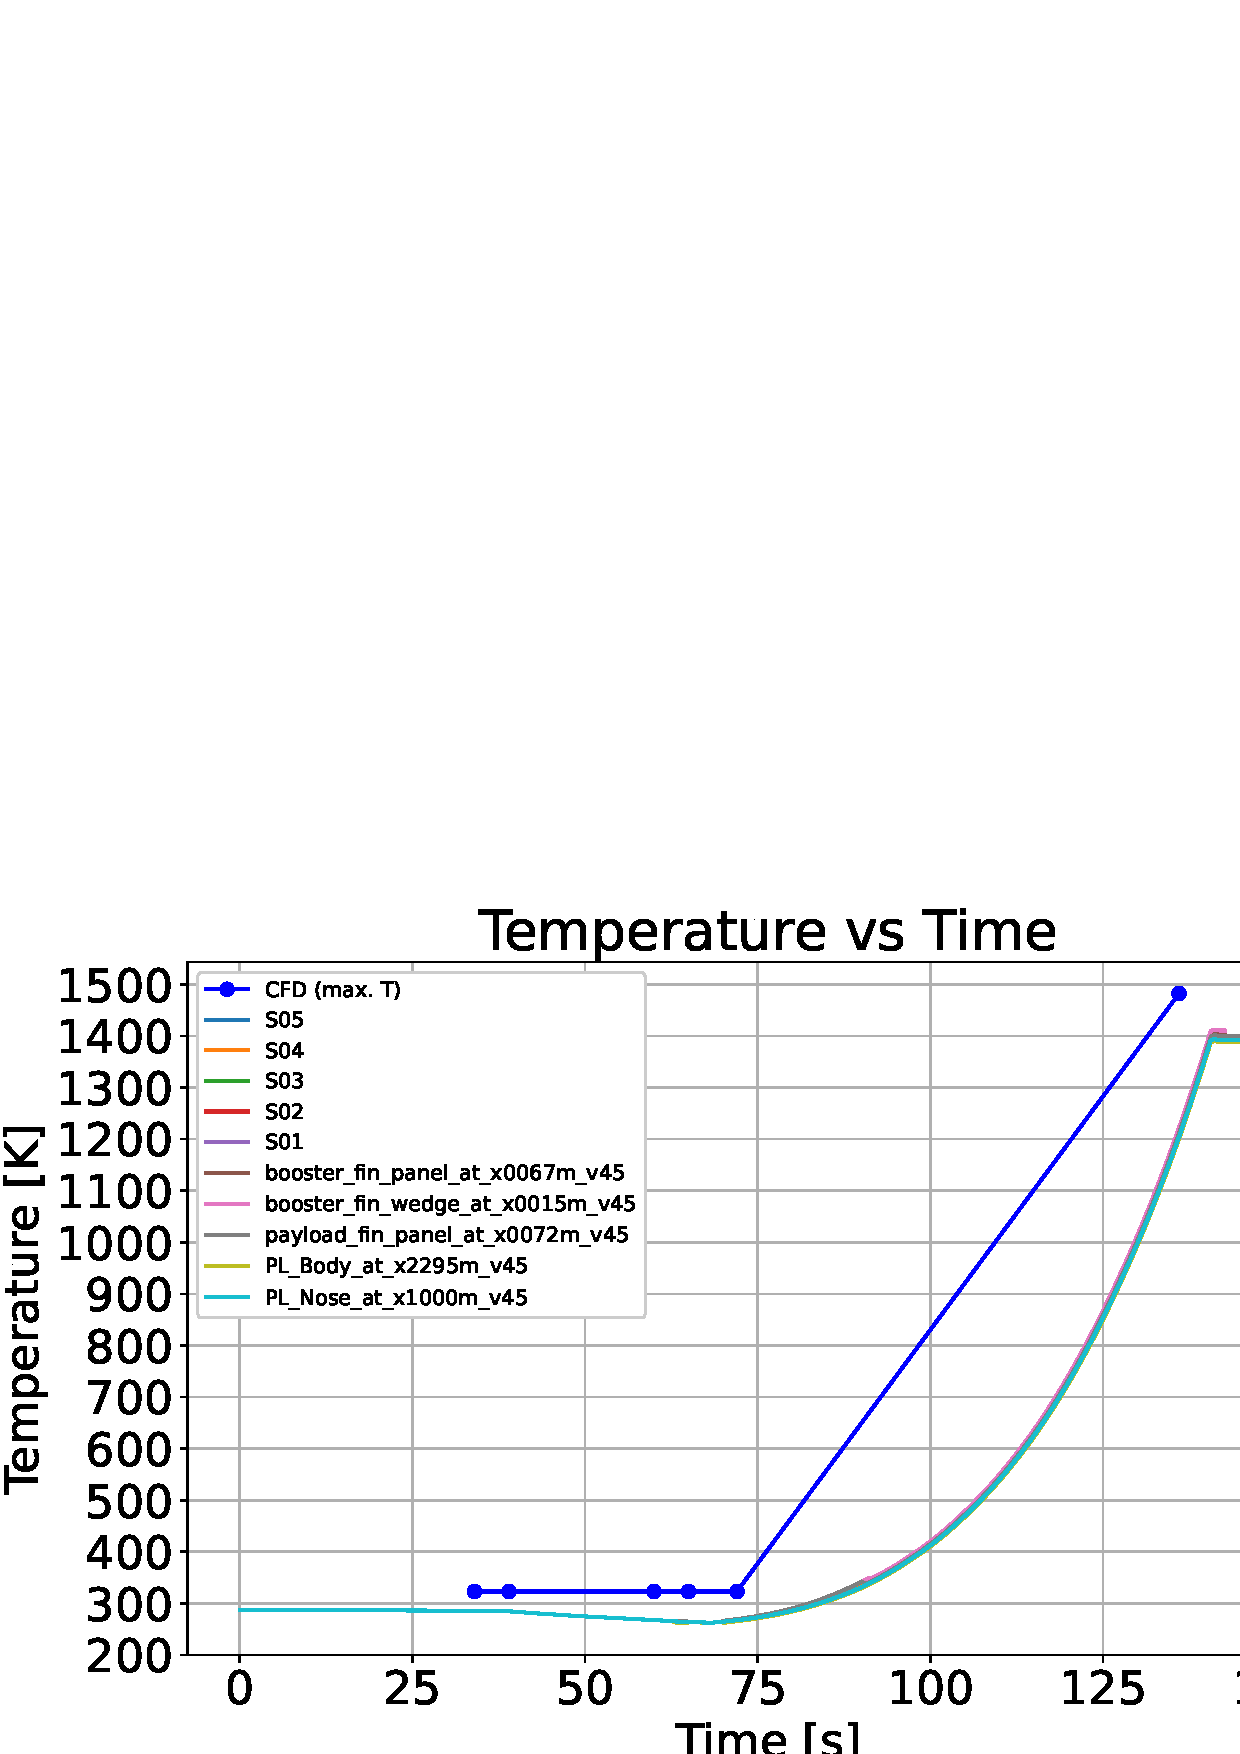
\includegraphics[width=\linewidth]{figs/oldHF/temperature.png}
%    \caption{Wall temperature (first cell) extracted from CFD for several point along the flight trajectory. The S01-S05 are from~\url{https://git2.gspacetech.com/systems/analysis-reviews/-/issues/1}.}
%    \label{fig:Tw}
%\end{figure}
%
%\begin{figure}[H]
%    \centering
%    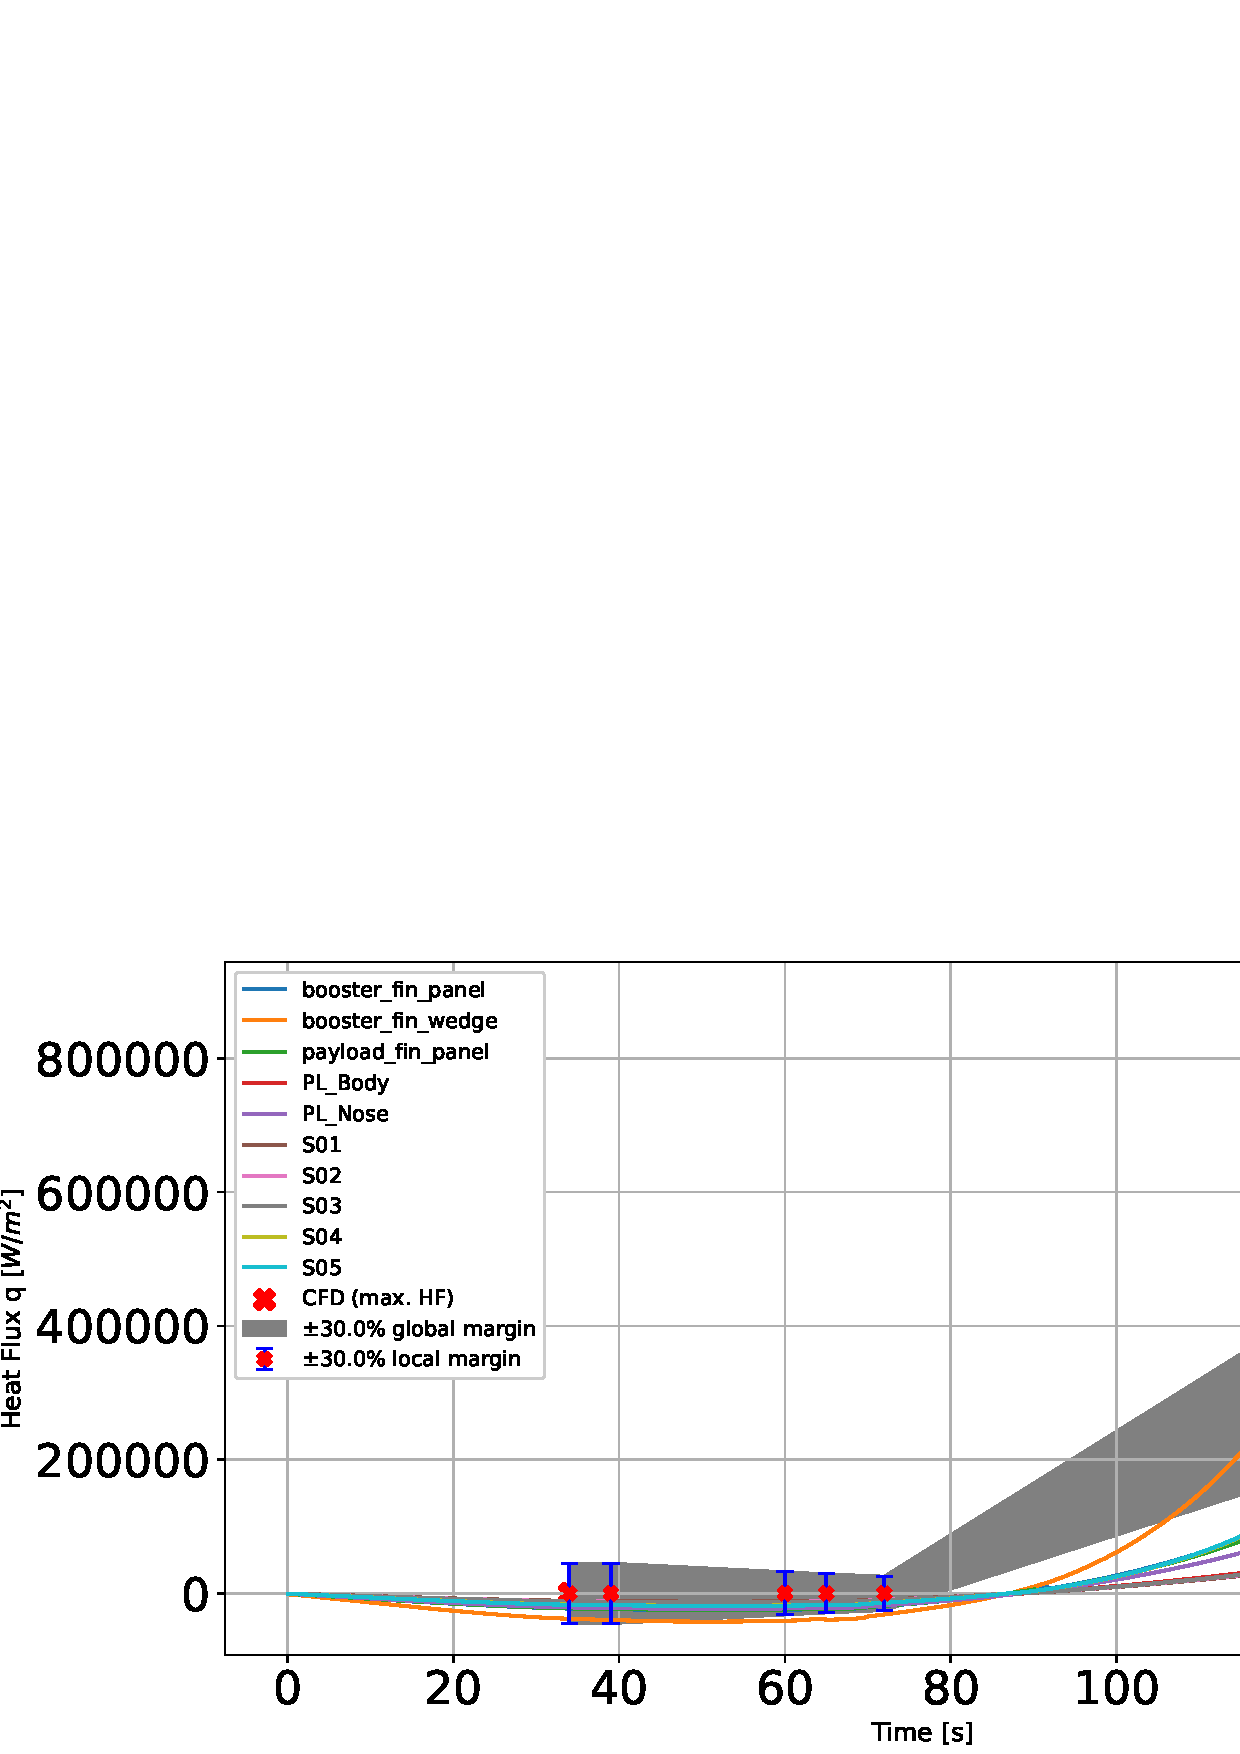
\includegraphics[width=\linewidth]{figs/oldHF/heatflux.png}
%    \caption{Wall heat flux computed from CFD for several point along the flight trajectory. The blue line represents the maximum heat flux among all wall points at each time. The S01-S05 are from~\url{https://git2.gspacetech.com/systems/analysis-reviews/-/issues/1}. The value of the total surface heat flux has a maximum on the leading edge of the fin equal to $q_{fin} \approx 200000~W/m^2$ which appears to be significantly lower than the value (orange line) predicted by DATCOM and almost inside the lower bound defined on top of OpenFOAM solutions. By comparing these legacy values with those from Table~\ref{tab:full_aeroheat_data_onon}, it can be observed that the values of heat flux for the other surfaces, such as the booster, appear to be much lower than the DATCOM predictions.}
%    \label{fig:qw}
%\end{figure}
%
%%\begin{figure}[H]
%%    \centering
%%    \includegraphics[width=0.9\linewidth]{figs/oldHF/legacy_Tref.png}
%%    \caption{\textbf{Wall temperature on the base} section computed from CFD on the base section %at $t=136s$ for \textbf{jetOFF/jetON} configurations. The S01-S05 are from~\url{https://%git2.gspacetech.com/systems/analysis-reviews/-/issues/1}.}
%%    \label{fig:q}
%%\end{figure}
%
%\begin{figure}[H]
%    \centering
%    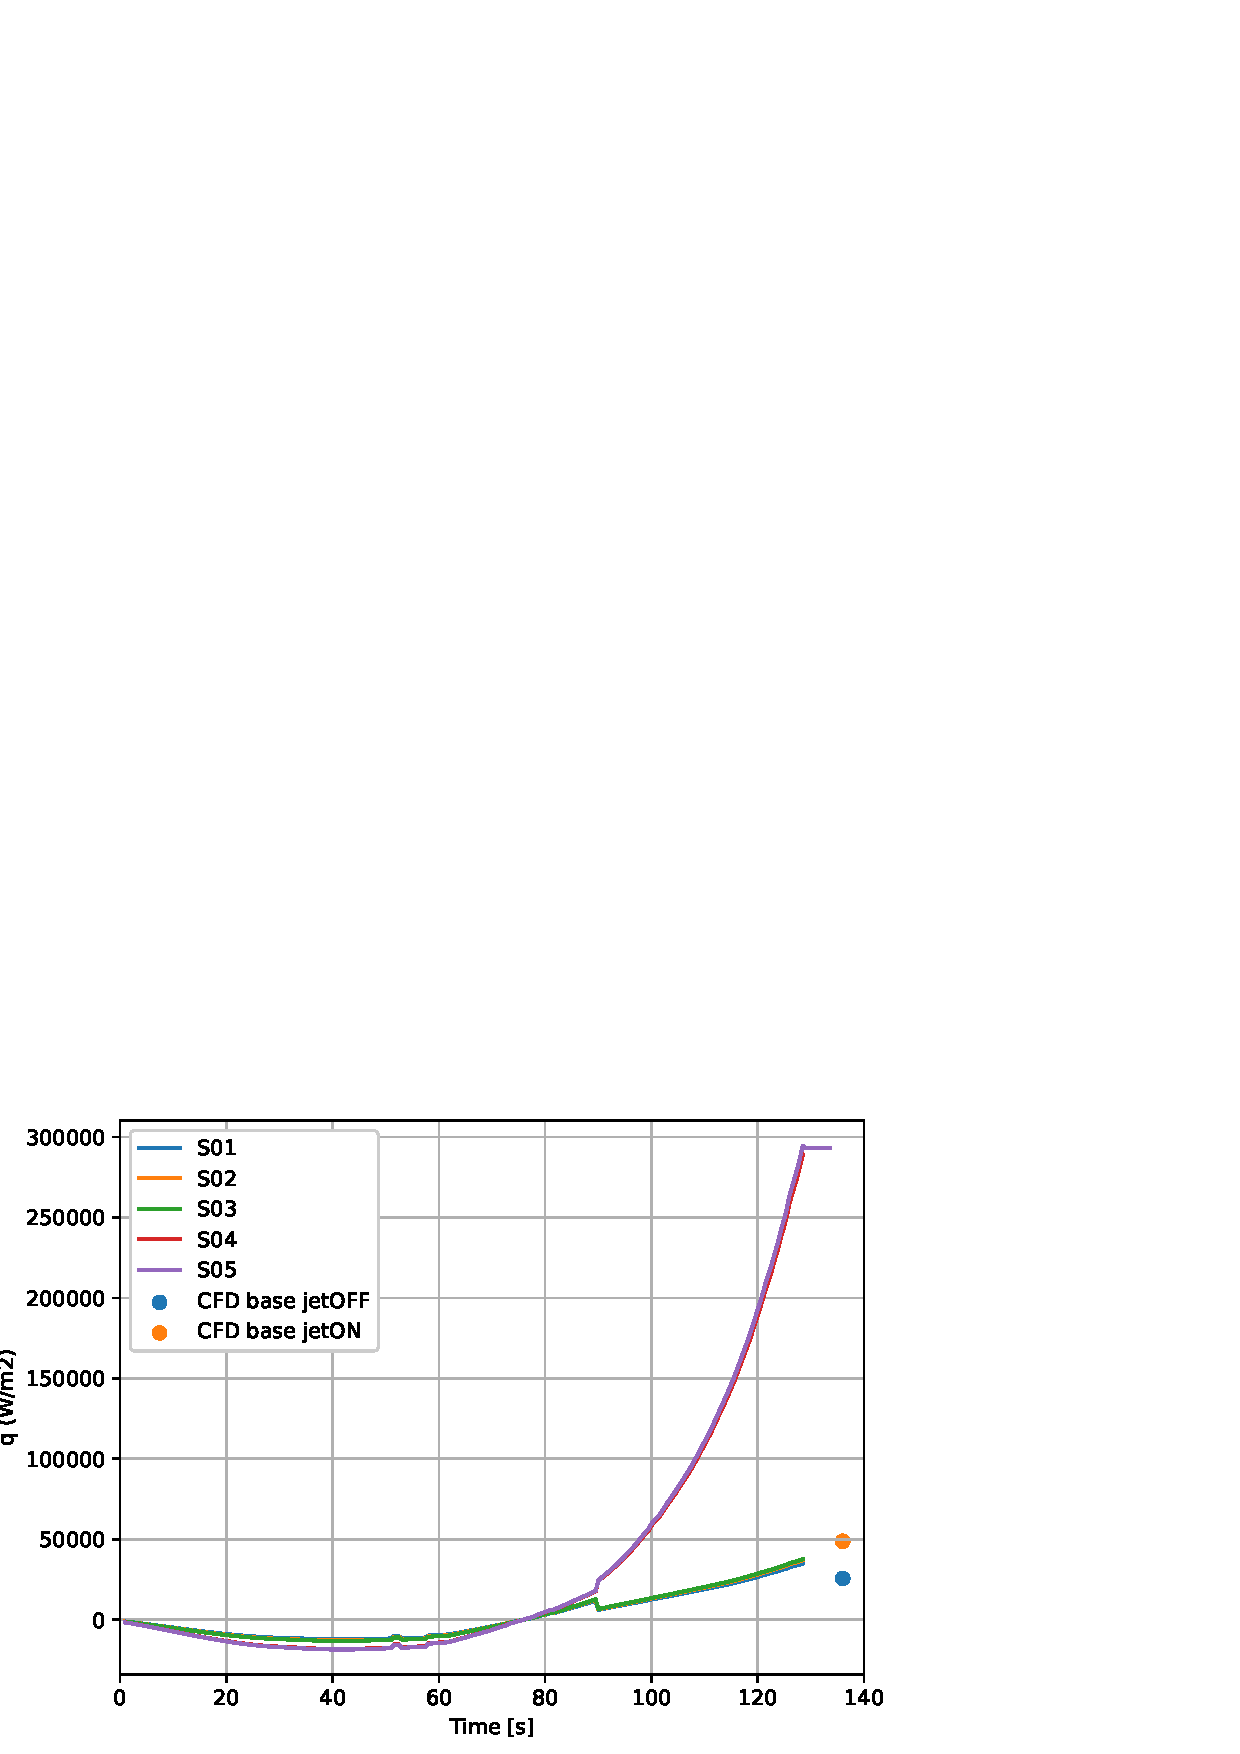
\includegraphics[width=0.9\linewidth]{figs/oldHF/legacy_q.png}
%    \caption{\textbf{Wall heat flux on the base} section computed from CFD  at $t=136s$ for \textbf{jetOFF/jetON} configurations. The S01-S05 are from~\url{https://git2.gspacetech.com/systems/analysis-reviews/-/issues/1}. \hl{Note that the new results for \textbf{jetON/VernierON} provide a an average value of the base heat flux of $q_{base} \approx 40000~W/m^2$ which is in good agreement with previous results.}}
%    \label{fig:qbase}
%\end{figure}
%%
%\begin{figure}[H]
%    \centering
%    \includegraphics[width=\linewidth]{figs/QvsTime.pdf}
%    \caption{Area-averaged heat flux in different patches in time for Charon jetON/VernierOFF configuration.}
%    \label{fig:QvsTime}
%\end{figure}
%%
%Numerical results obtained from CFD simulations appear to be in reasonable agreement with aerothermal analysis previously performed in~\url{https://git2.gspacetech.com/systems/analysis-reviews/-/issues/1} even for the worst case occurring at $=136s$.

%%%%%%%%%%%%%%%%%%%%%%%%%%%%%%%%%%%%%%%%%%%%
\section{Conclusions}\label{sec:conclusions}
%%%%%%%%%%%%%%%%%%%%%%%%%%%%%%%%%%%%%%%%%%%%
In this work package an aerothermodynamic analysis was conducted for the Charon vehicle. Numerical simulations were performed in Fluent in order to calculated the aerodynamic coefficients for the jetON (with plume) configuration. Aerodynamic loads and aeroheating fluxes were estimated on the base, fin and raceway regions as well as on the whole surface wall.

The following observations apply:

\begin{itemize}
\item \hl{Any reported $C_N$, $C_M$ coefficient value is \textbf{not representative} (while $C_A$ it is) of the full vehicle configuration as only one-quarter model was simulated.}
\item \hl{The aerothermal loads are \textbf{not reliable} as the numerical simulations did not converged for the energy equations and the wall heat flux field presents defected cell spikes which wrongly steer the average values.}
\end{itemize}

%%%%%%%%%%%%%%%%%%%%%%%%%%%%%%%%%%%%%%%%%%%%%%%%%%%%%%%%%%%%%%%%%%%%%%%
\section{Appendix: Nozzle exit flow conditions from RPA}\label{sec:RPA}
%%%%%%%%%%%%%%%%%%%%%%%%%%%%%%%%%%%%%%%%%%%%%%%%%%%%%%%%%%%%%%%%%%%%%%%

\foreach \filename/\captiontext in {
    0sec.txt/{$t = 0 s$}, % actually +8 sec after ramp up 
    35sec.txt/{$t = 35 s$},
    39.3sec.txt/{$t = 39.3 s$},
    50sec.txt/{$t = 50 s$},
    60.6sec.txt/{$t = 60.6 s$},
    65.9sec.txt/{$t = 65.9 s$},
    72.7sec.txt/{$t = 72.7 s$},
    93s.txt/{$t = 93 s$},
    110s.txt/{$t = 110 s$},
    122s.txt/{$t = 122 s$},
    136.7sec.txt/{$t = 136.7 s$}
} {
    \lstinputlisting[
        caption=\captiontext,
        label=lst:\captiontext
    ]{data/\filename}
}

% Signature
\vspace{\fill}
\begin{center}
    \hspace*{9.0cm} \LARGE \textbf{Lorenzo Campoli} \\
    \hspace*{9.0cm}\includegraphics[width=0.45\textwidth]{signature/signature0.png}
\end{center}

\vspace*{-1.0cm}

\hspace*{9.0cm}\textbf{Senior Systems Modelling Engineer}

\hspace*{9.0cm}\textbf{Gilmour Space Technologies}

\hspace*{9.0cm}\textbf{lorenzo.campoli@gspace.com}

\newpage
\bibliography{refs/refs}
\bibliographystyle{unsrt}

\end{document}